\chapter{Prezentacja projektu}
Rozdział zawiera zdjęcie i opisy przedstawiające działanie aplikacji mobilnej i strony internetowej.


\section{Strona internetowa}
Rozdział przedstawia widoki i działanie strony internetowej.


\subsection{Logowanie}
Po uruchomieniu strony ukazuje się widok zawierający formularz logowania do strony internetowej. Po pomyślnym zalogowaniu użytkownik zostaje przekierowany do strony domowej.


\begin{figure}[H]
    \centering
    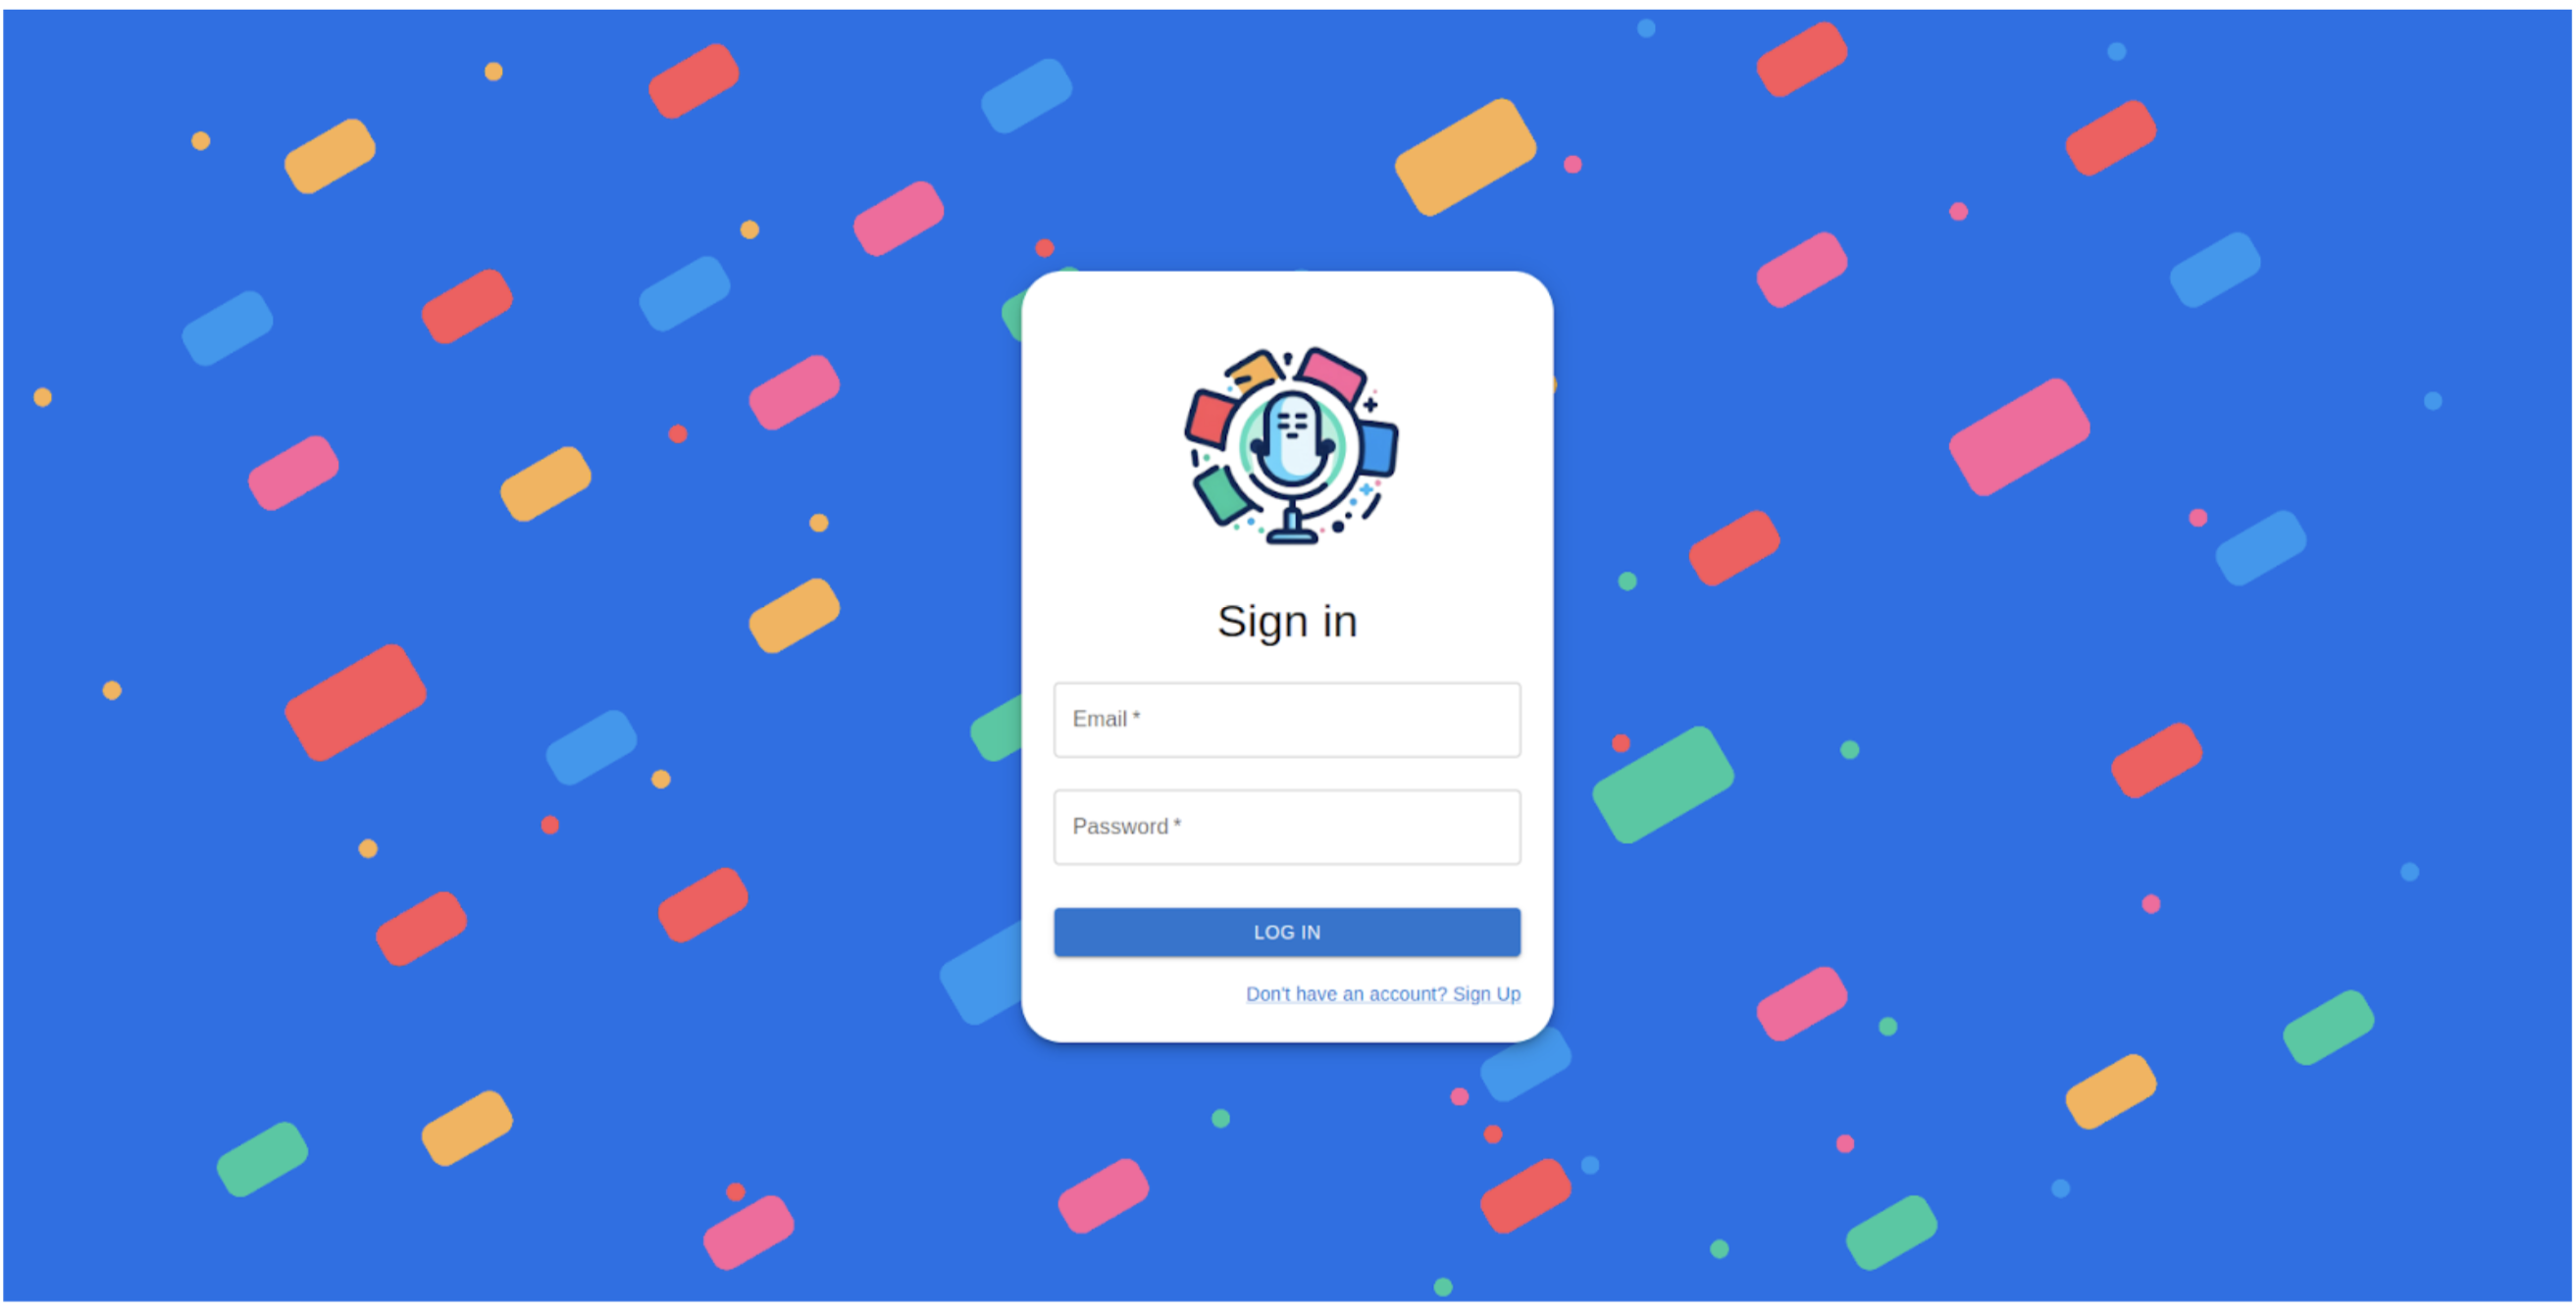
\includegraphics[width=0.9\textwidth]{chapters/chapter_10/images_web/web_login}
    \caption{Widok logowania.}
    \label{img:web_login}
\end{figure}


\begin{figure}[H]
    \centering
    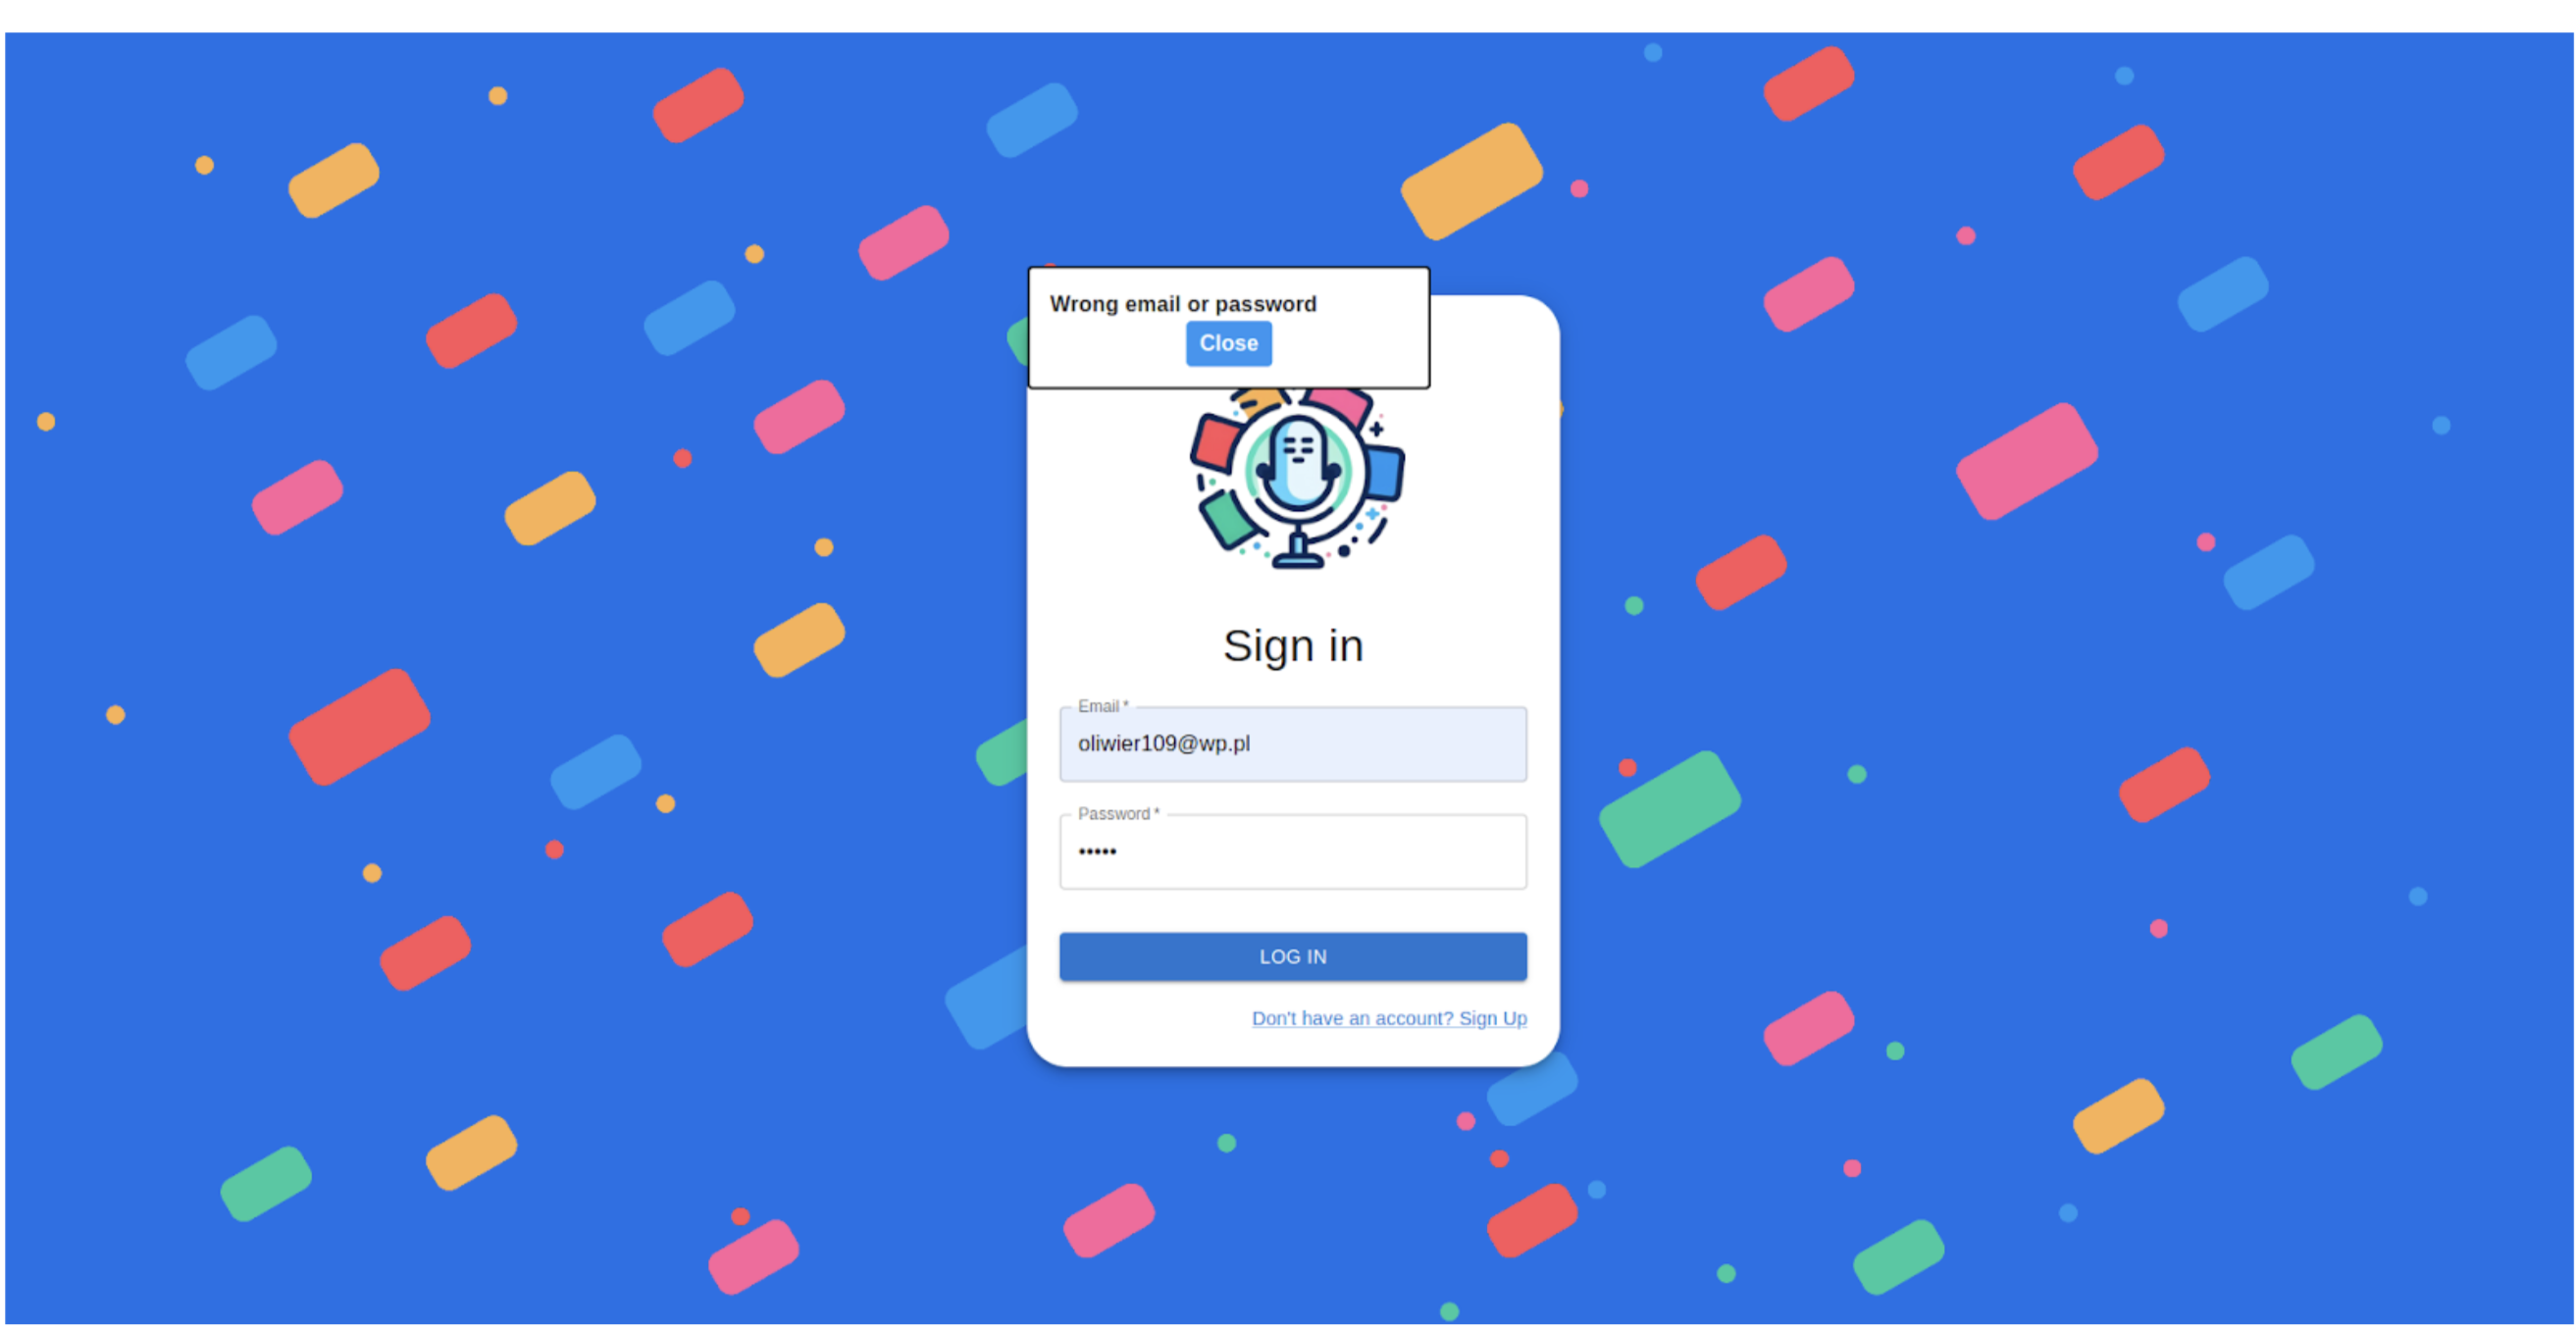
\includegraphics[width=0.9\textwidth]{chapters/chapter_10/images_web/web_login_2}
    \caption{Widok logowania po wpisaniu nieprawidłowych danych logowania.}
    \label{img:web_login_2}
\end{figure}


\subsection{Rejestracja}
Rejestracja pozwala na utworzenie konta potrzebnego do logowania.


\begin{figure}[H]
    \centering
    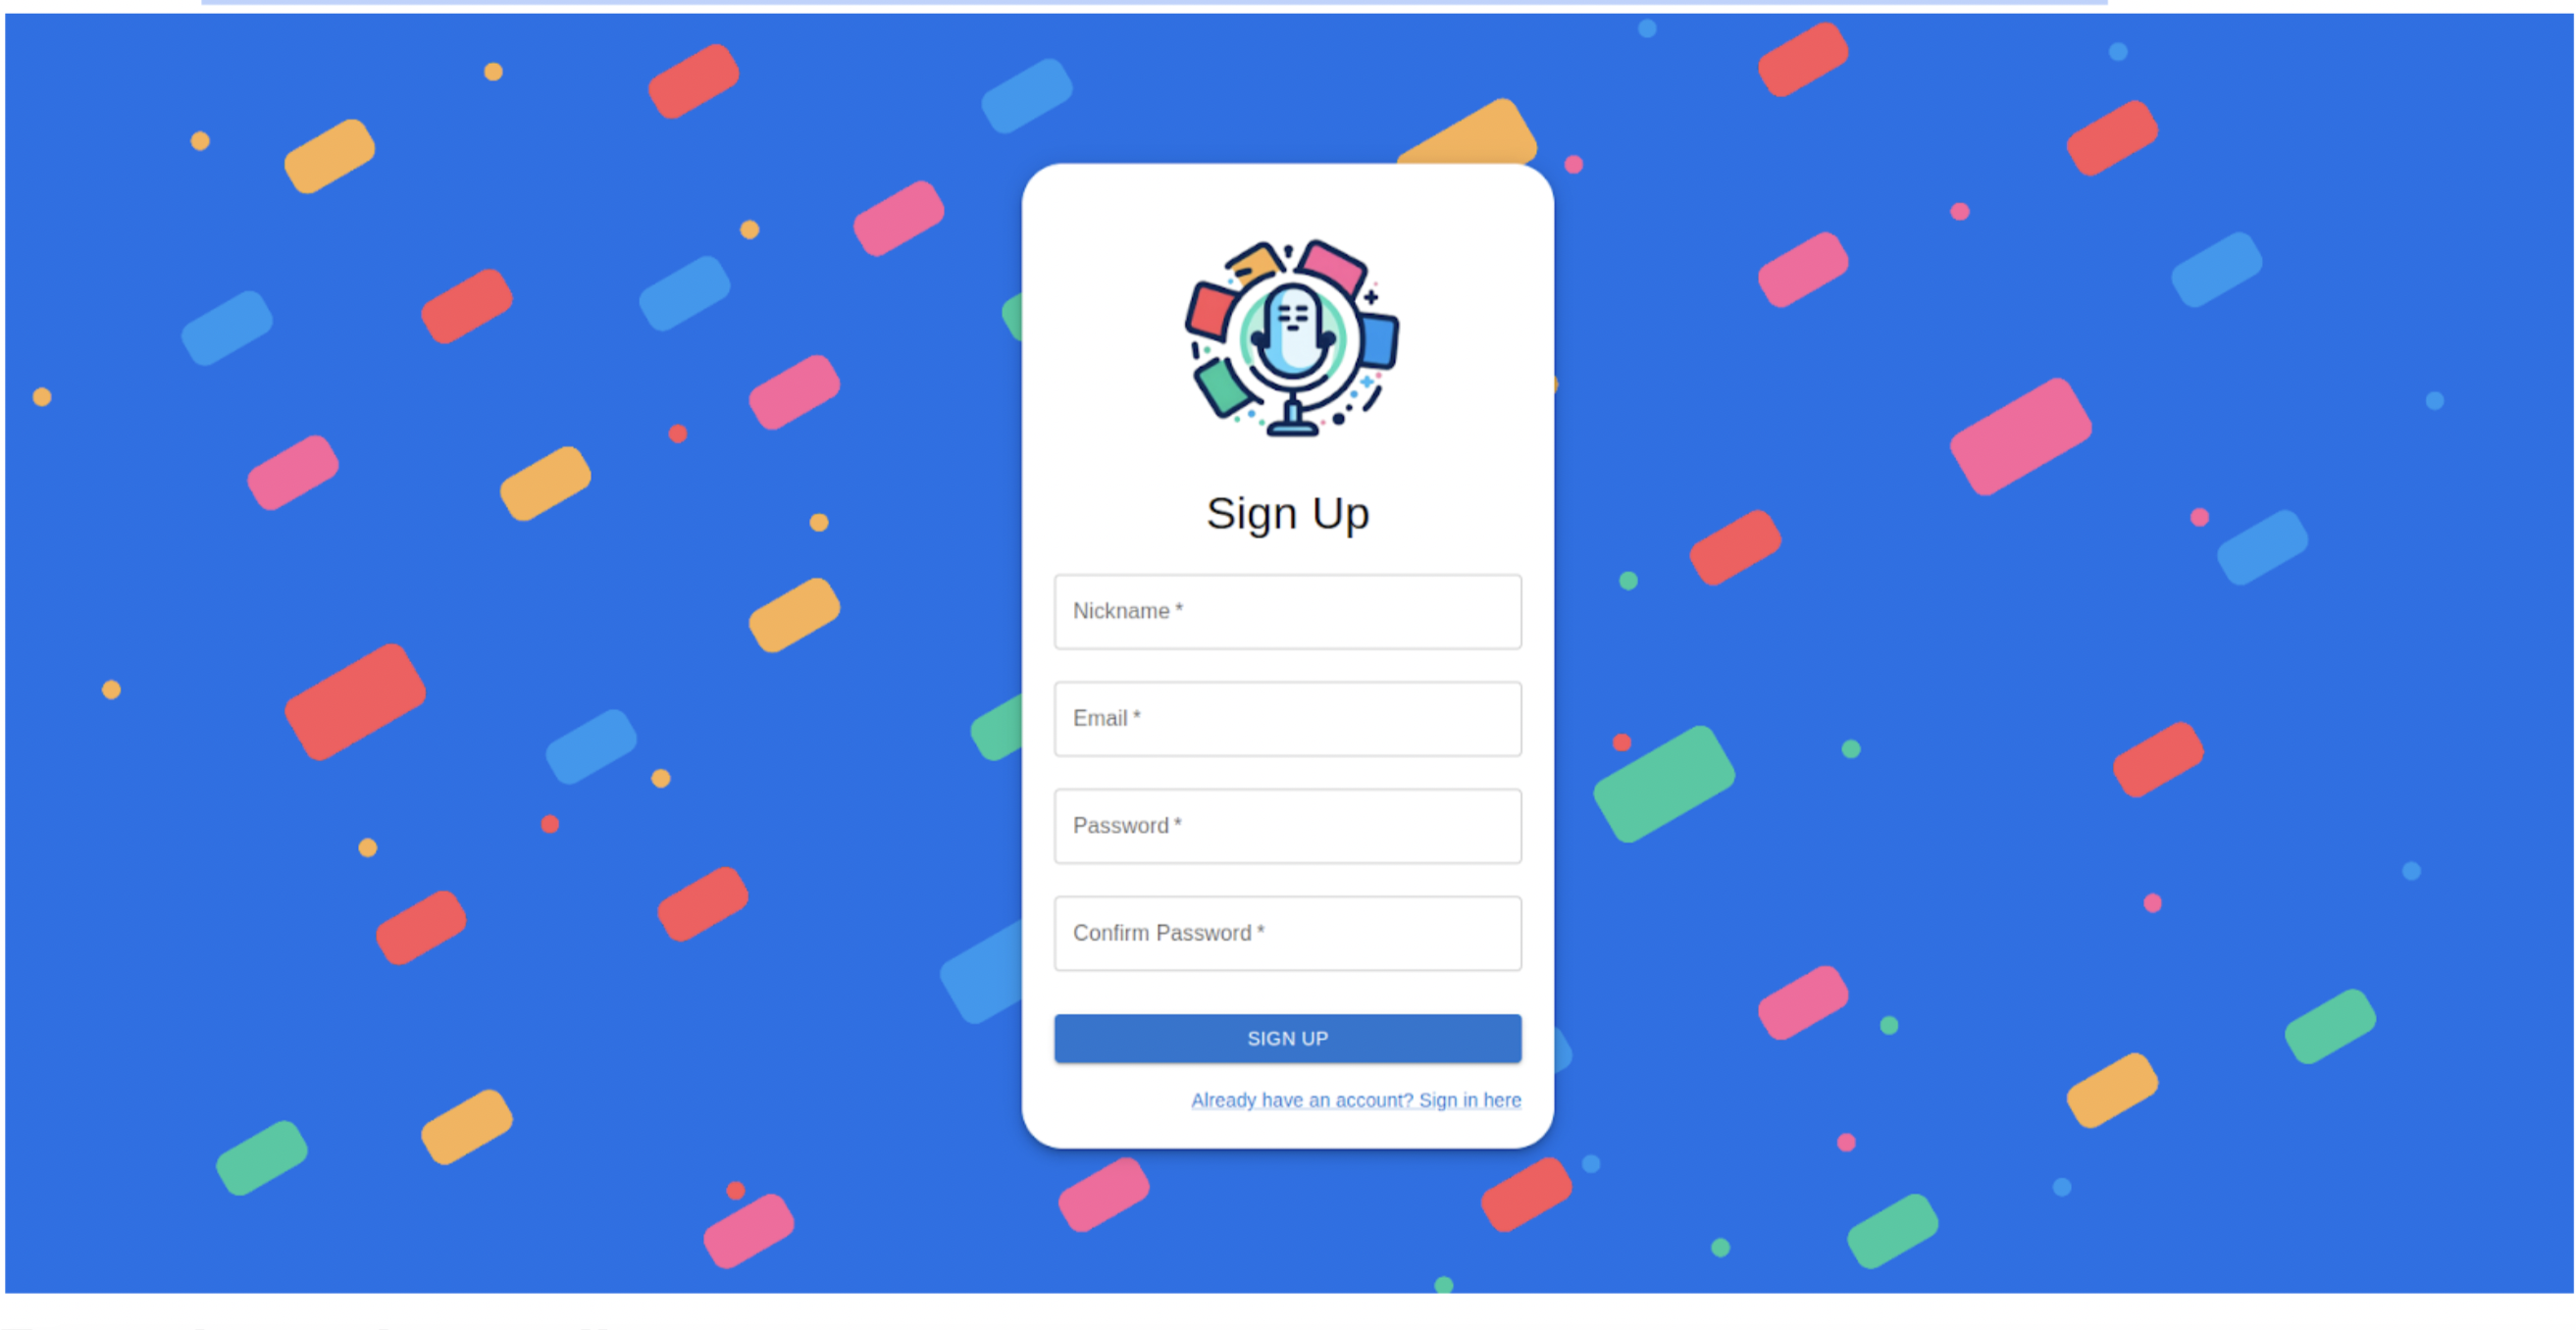
\includegraphics[width=0.9\textwidth]{chapters/chapter_10/images_web/web_register}
    \caption{Formularz rejestracji.}
    \label{img:web_register}
\end{figure}


\begin{figure}[H]
    \centering
    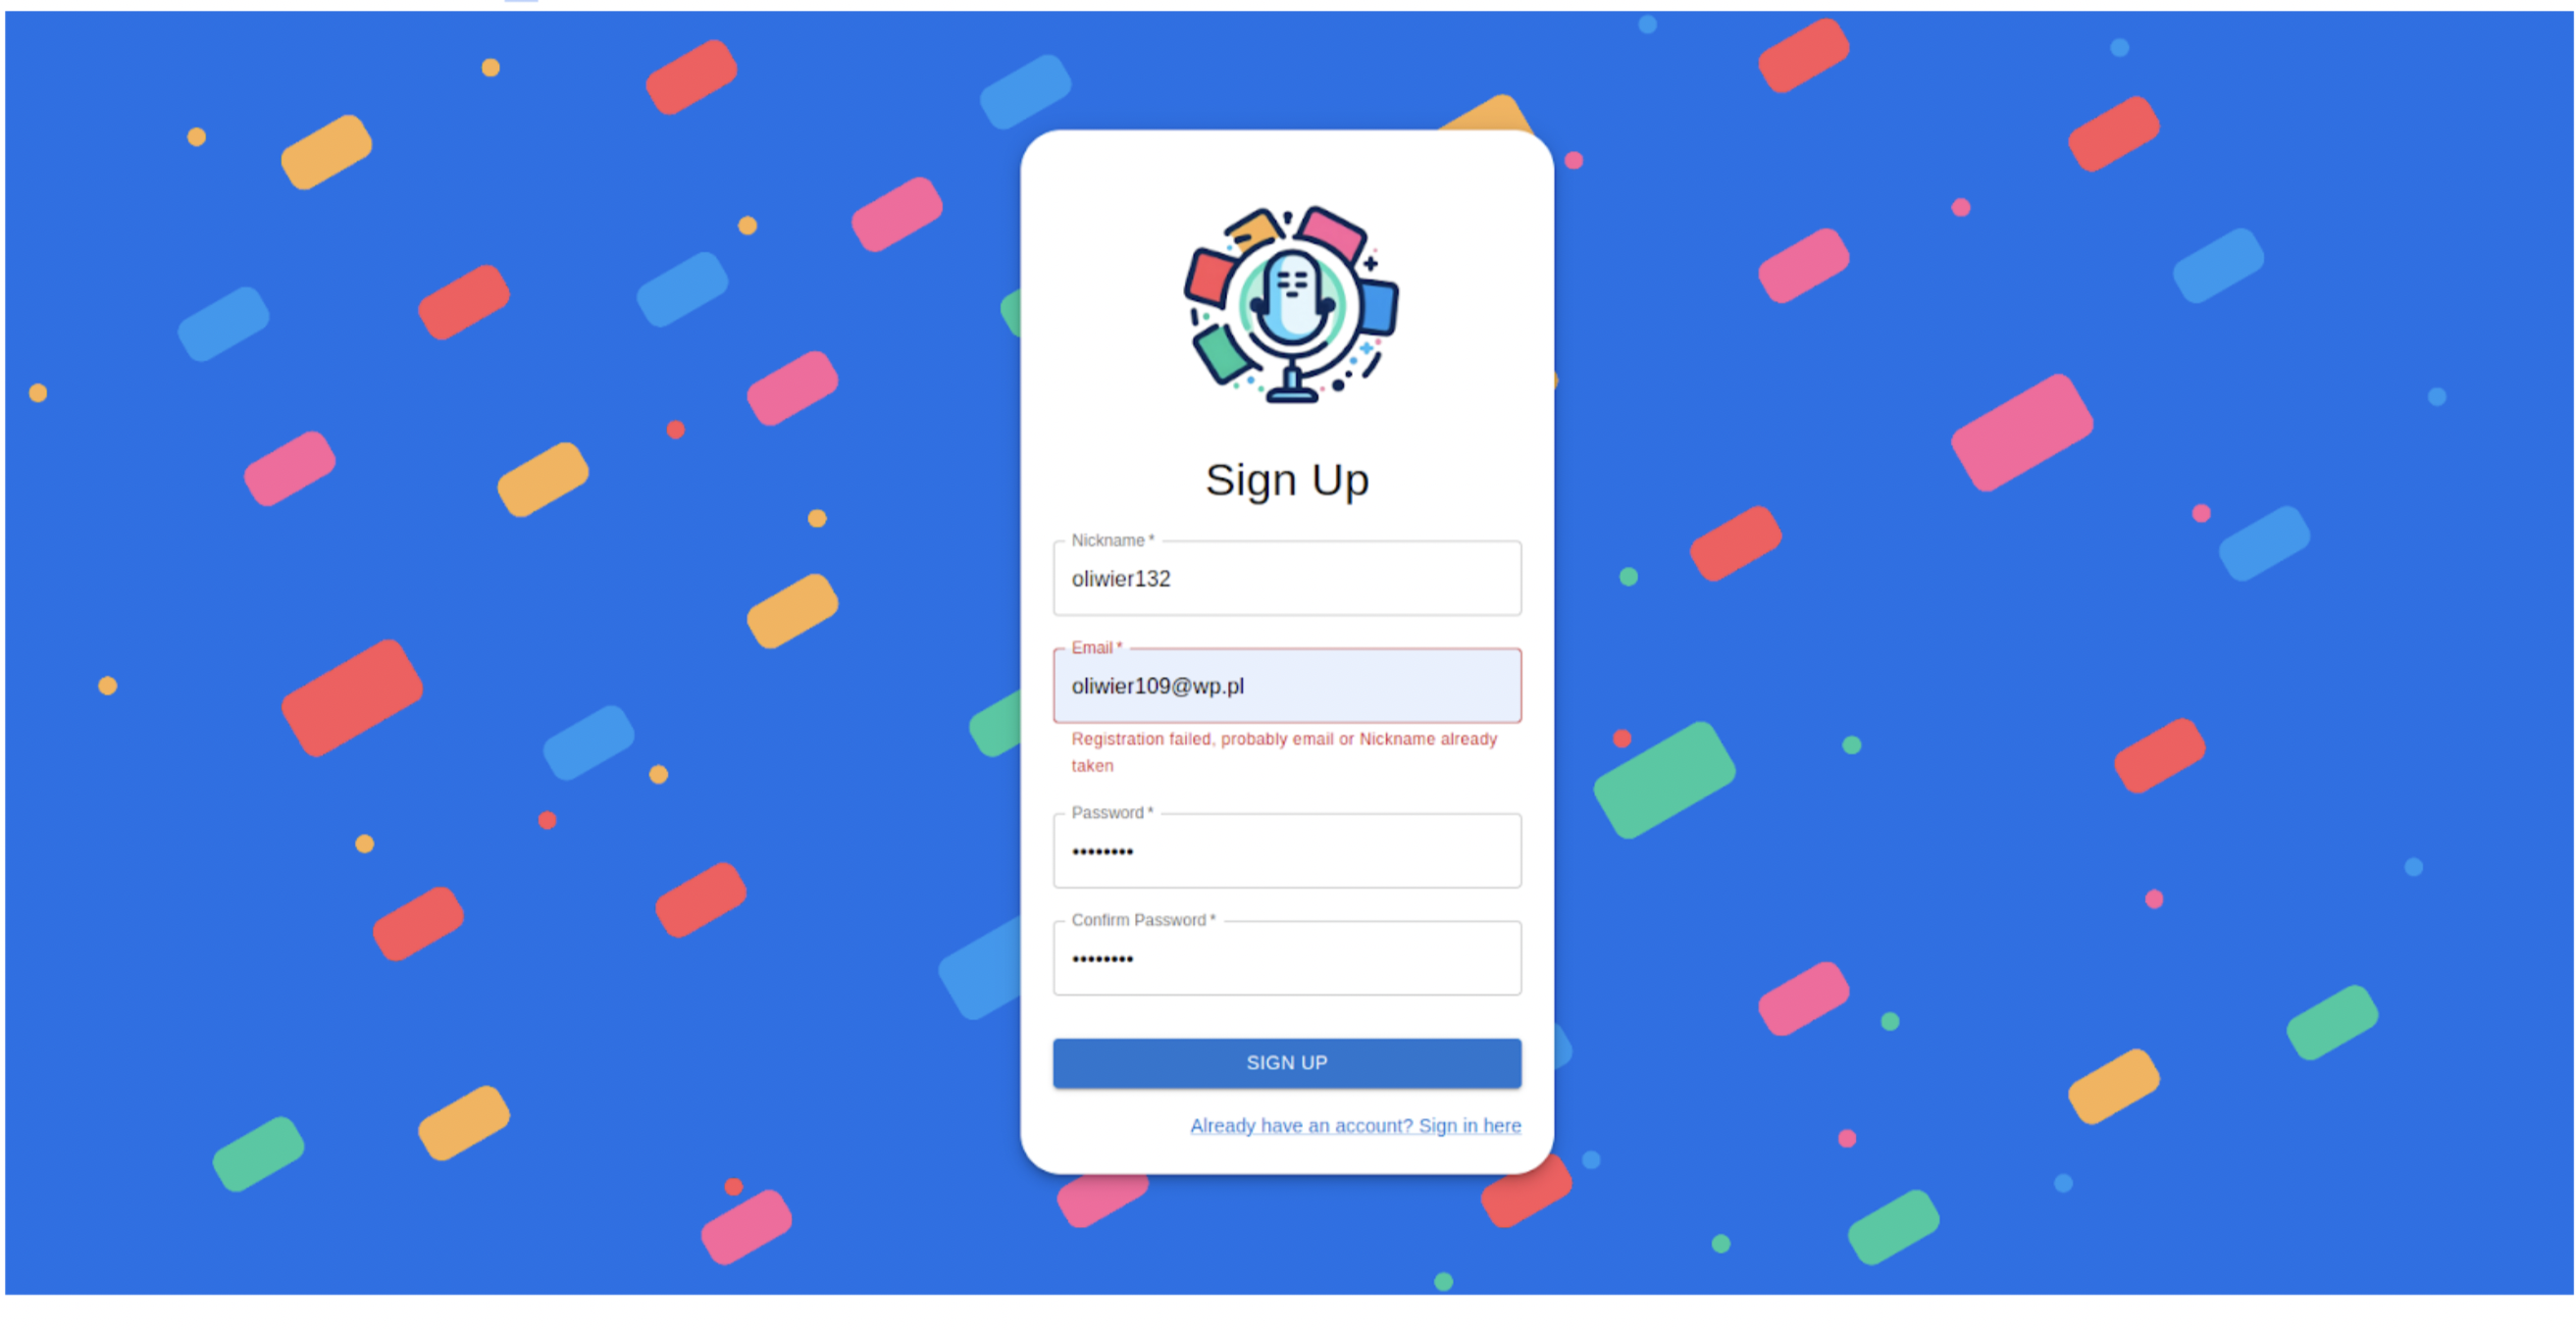
\includegraphics[width=0.9\textwidth]{chapters/chapter_10/images_web/web_register_2}
    \caption{Błąd po nieudanej rejestracji konta.}
    \label{img:web_register_2}
\end{figure}


\subsection{Strona domowa}
Po zalogowaniu użytkownik zostaje przekierowany do strony domowej. Na stronie domowej użytkownika możliwość wylogowania się lub może przejść do któregoś z podanych widoków:
\begin{itemize}
    \item Create Decks,
    \item My Decks,
    \item Public Decks,
    \item Profile,
    \item Ranking.
\end{itemize}


\begin{figure}[H]
    \centering
    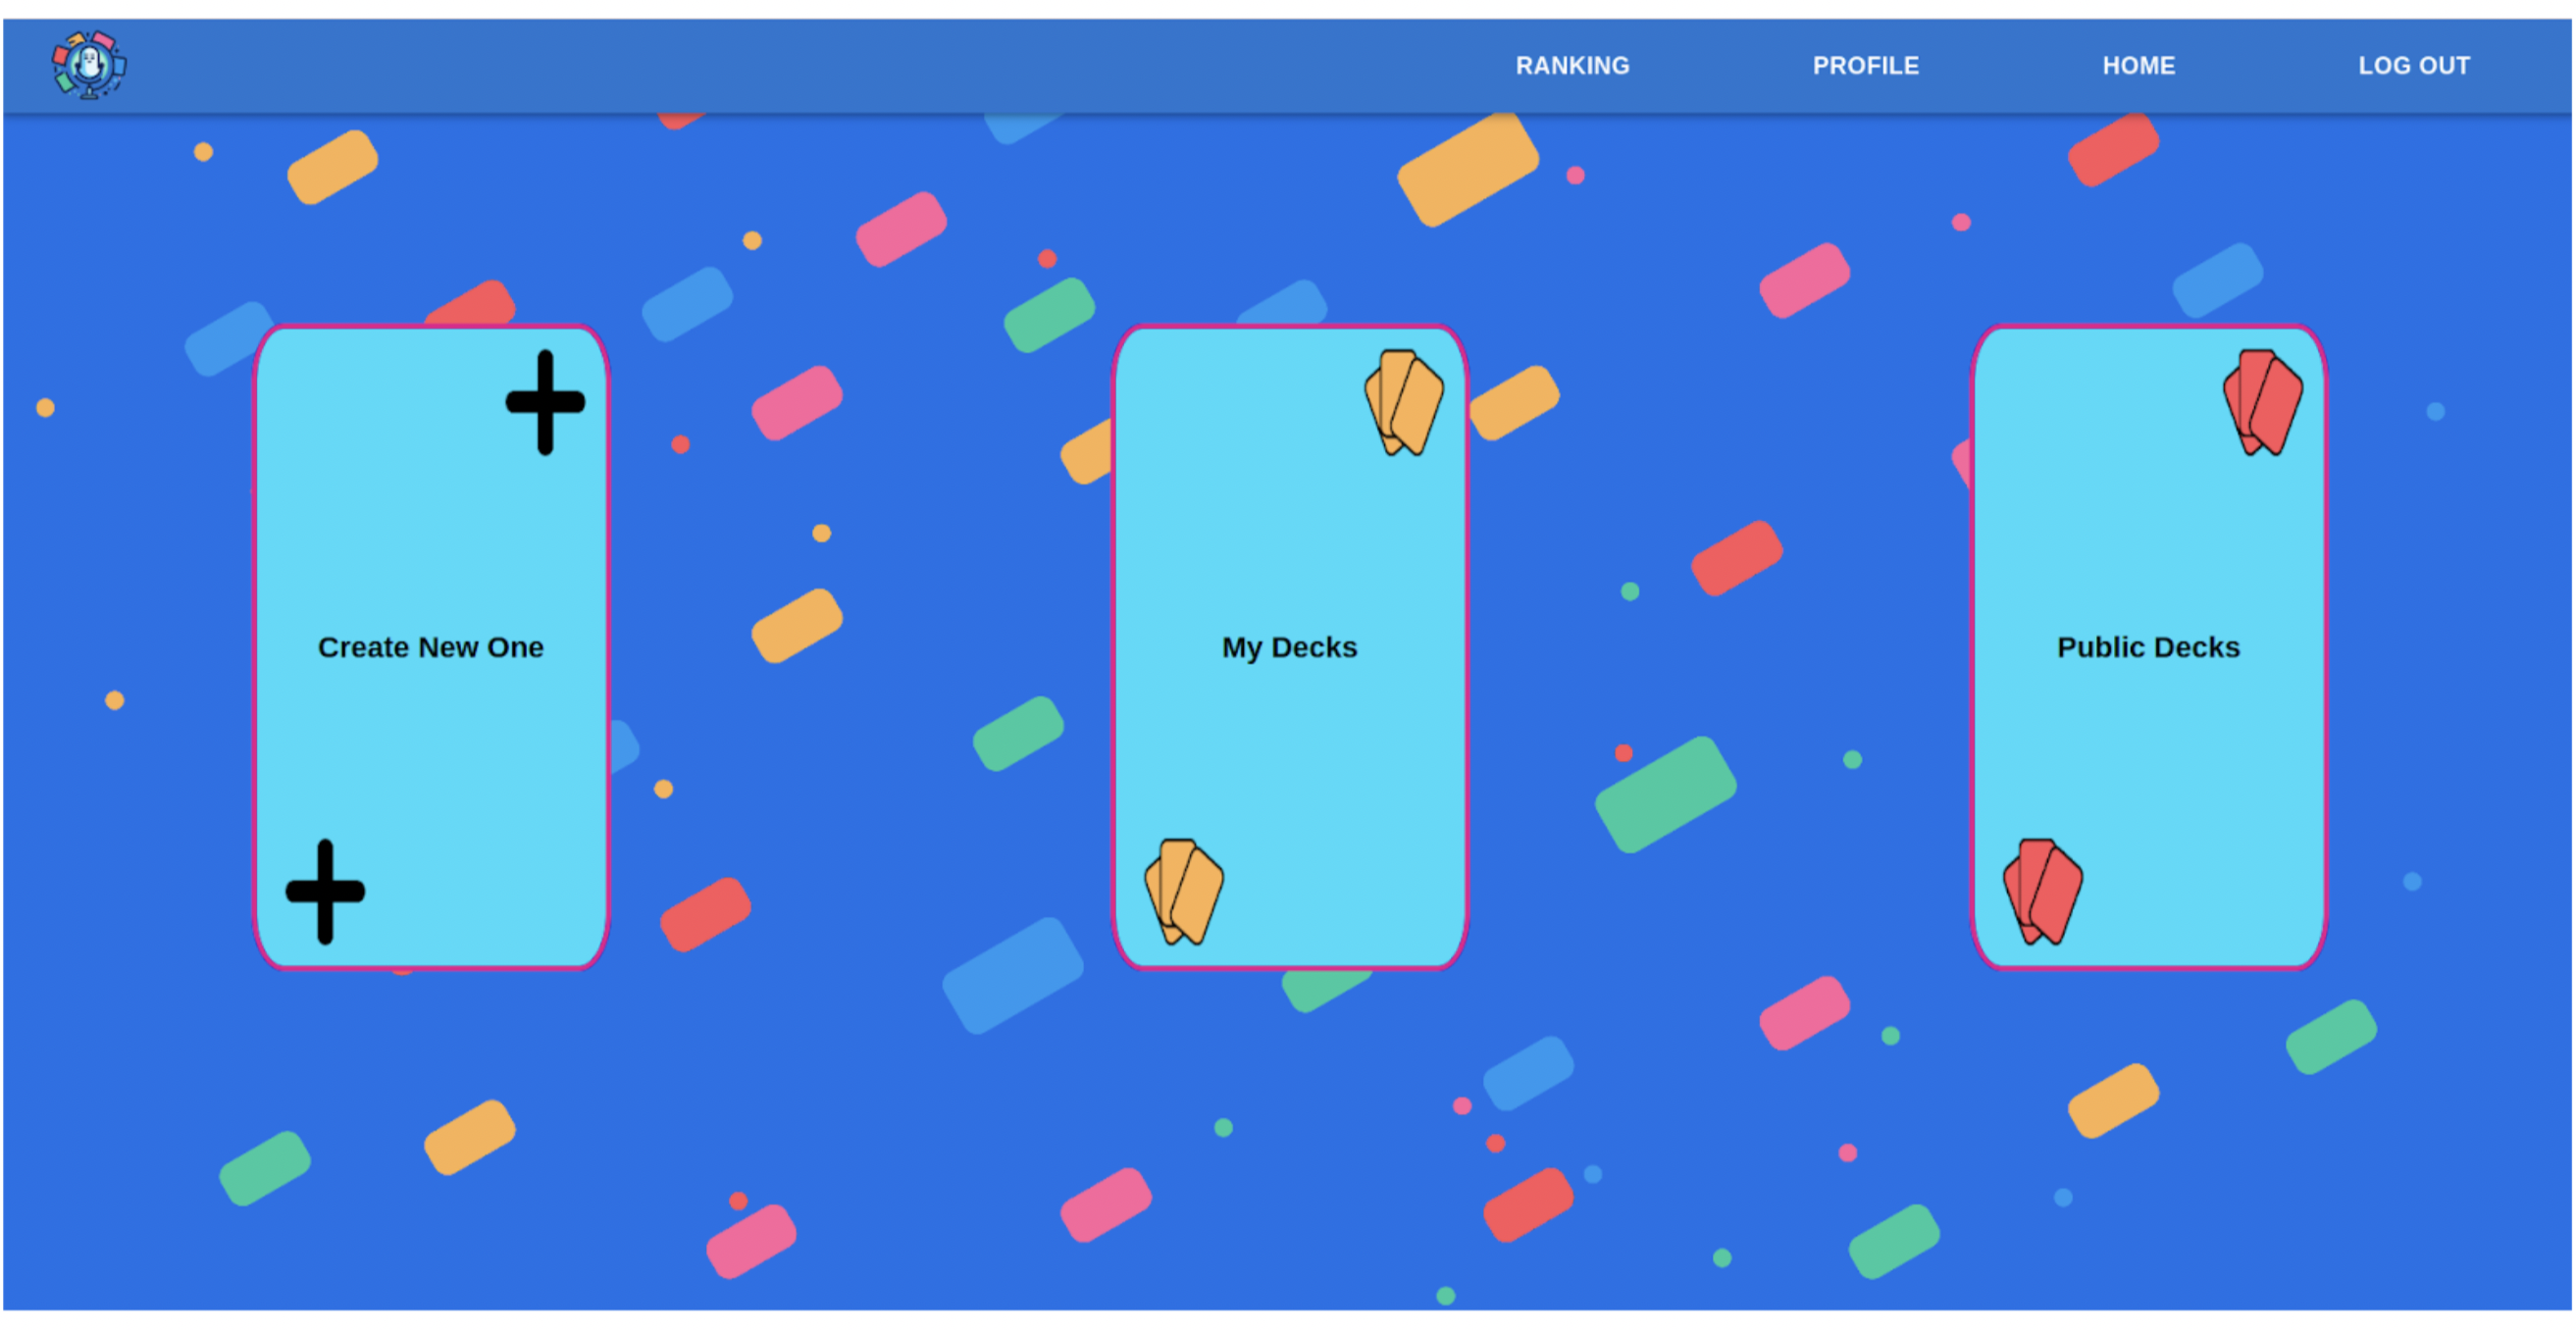
\includegraphics[width=0.9\textwidth]{chapters/chapter_10/images_web/web_home}
    \caption{Strona domowa.}
    \label{img:web_home}
\end{figure}


\subsection{Profil użytkownika}
Strona przedstawia profil użytkownika. Użytkownik ma możliwość zmiany swoich
danych, może usunąć konto, a także może przejść do widoku ze swoimi statystykami.


\begin{figure}[H]
    \centering
    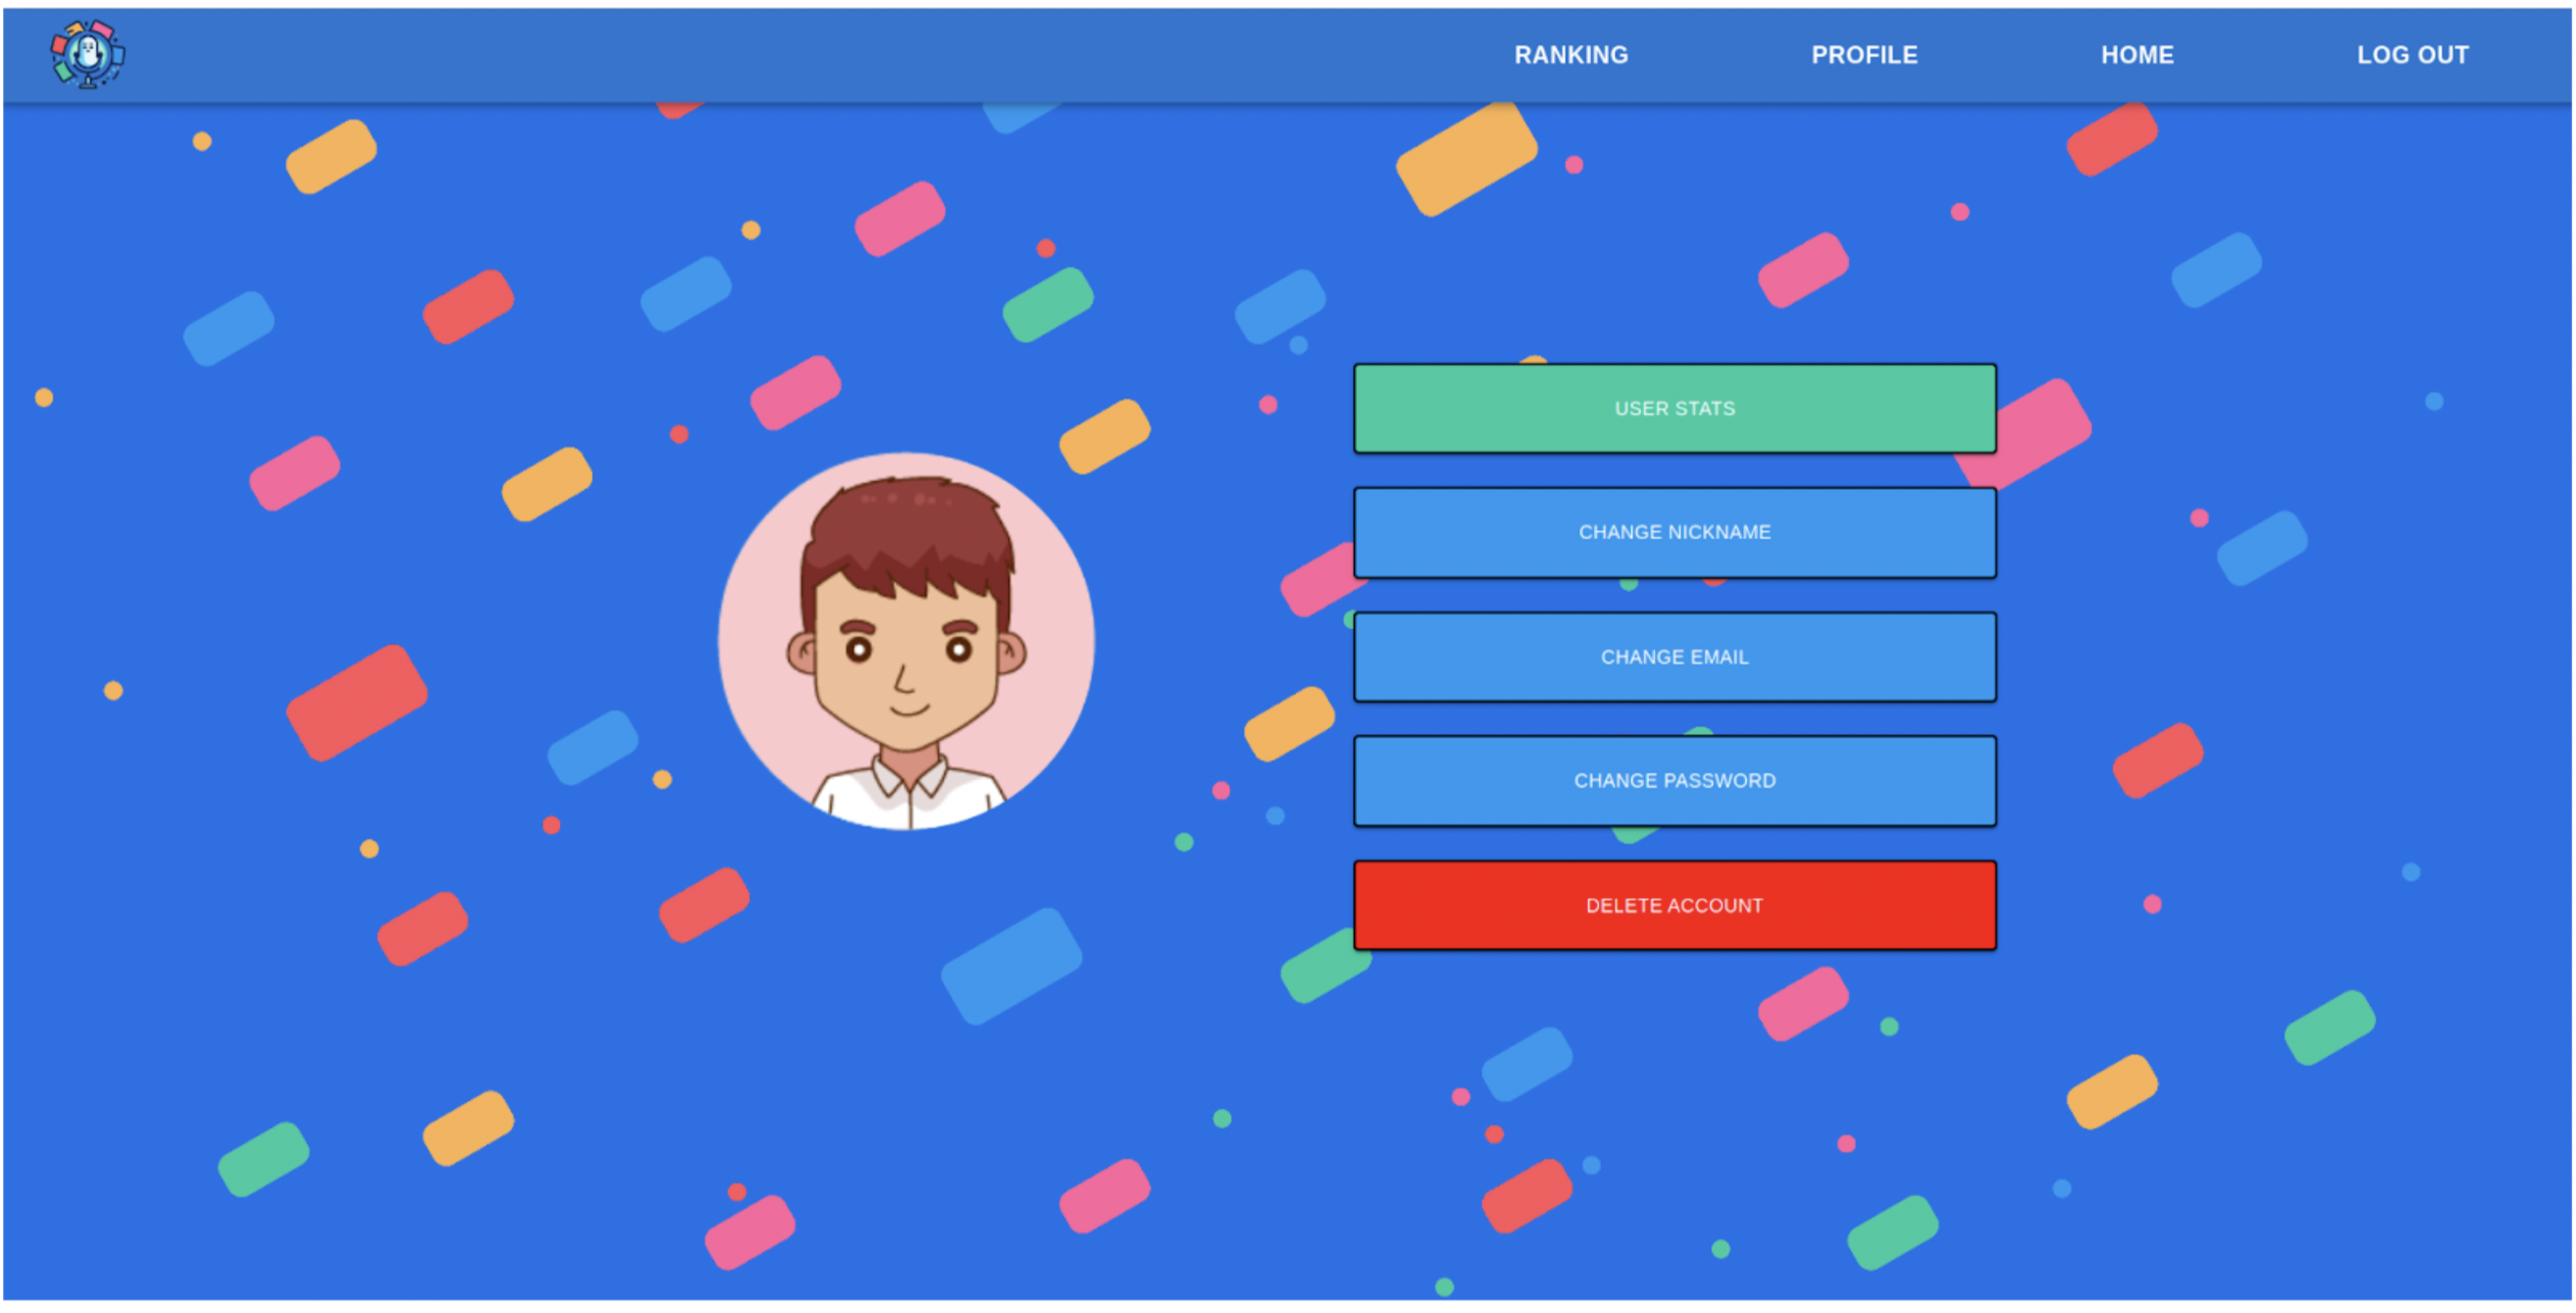
\includegraphics[width=0.9\textwidth]{chapters/chapter_10/images_web/web_profile}
    \caption{Profil użytkownika.}
    \label{img:web_profile}
\end{figure}


\begin{figure}[H]
    \centering
    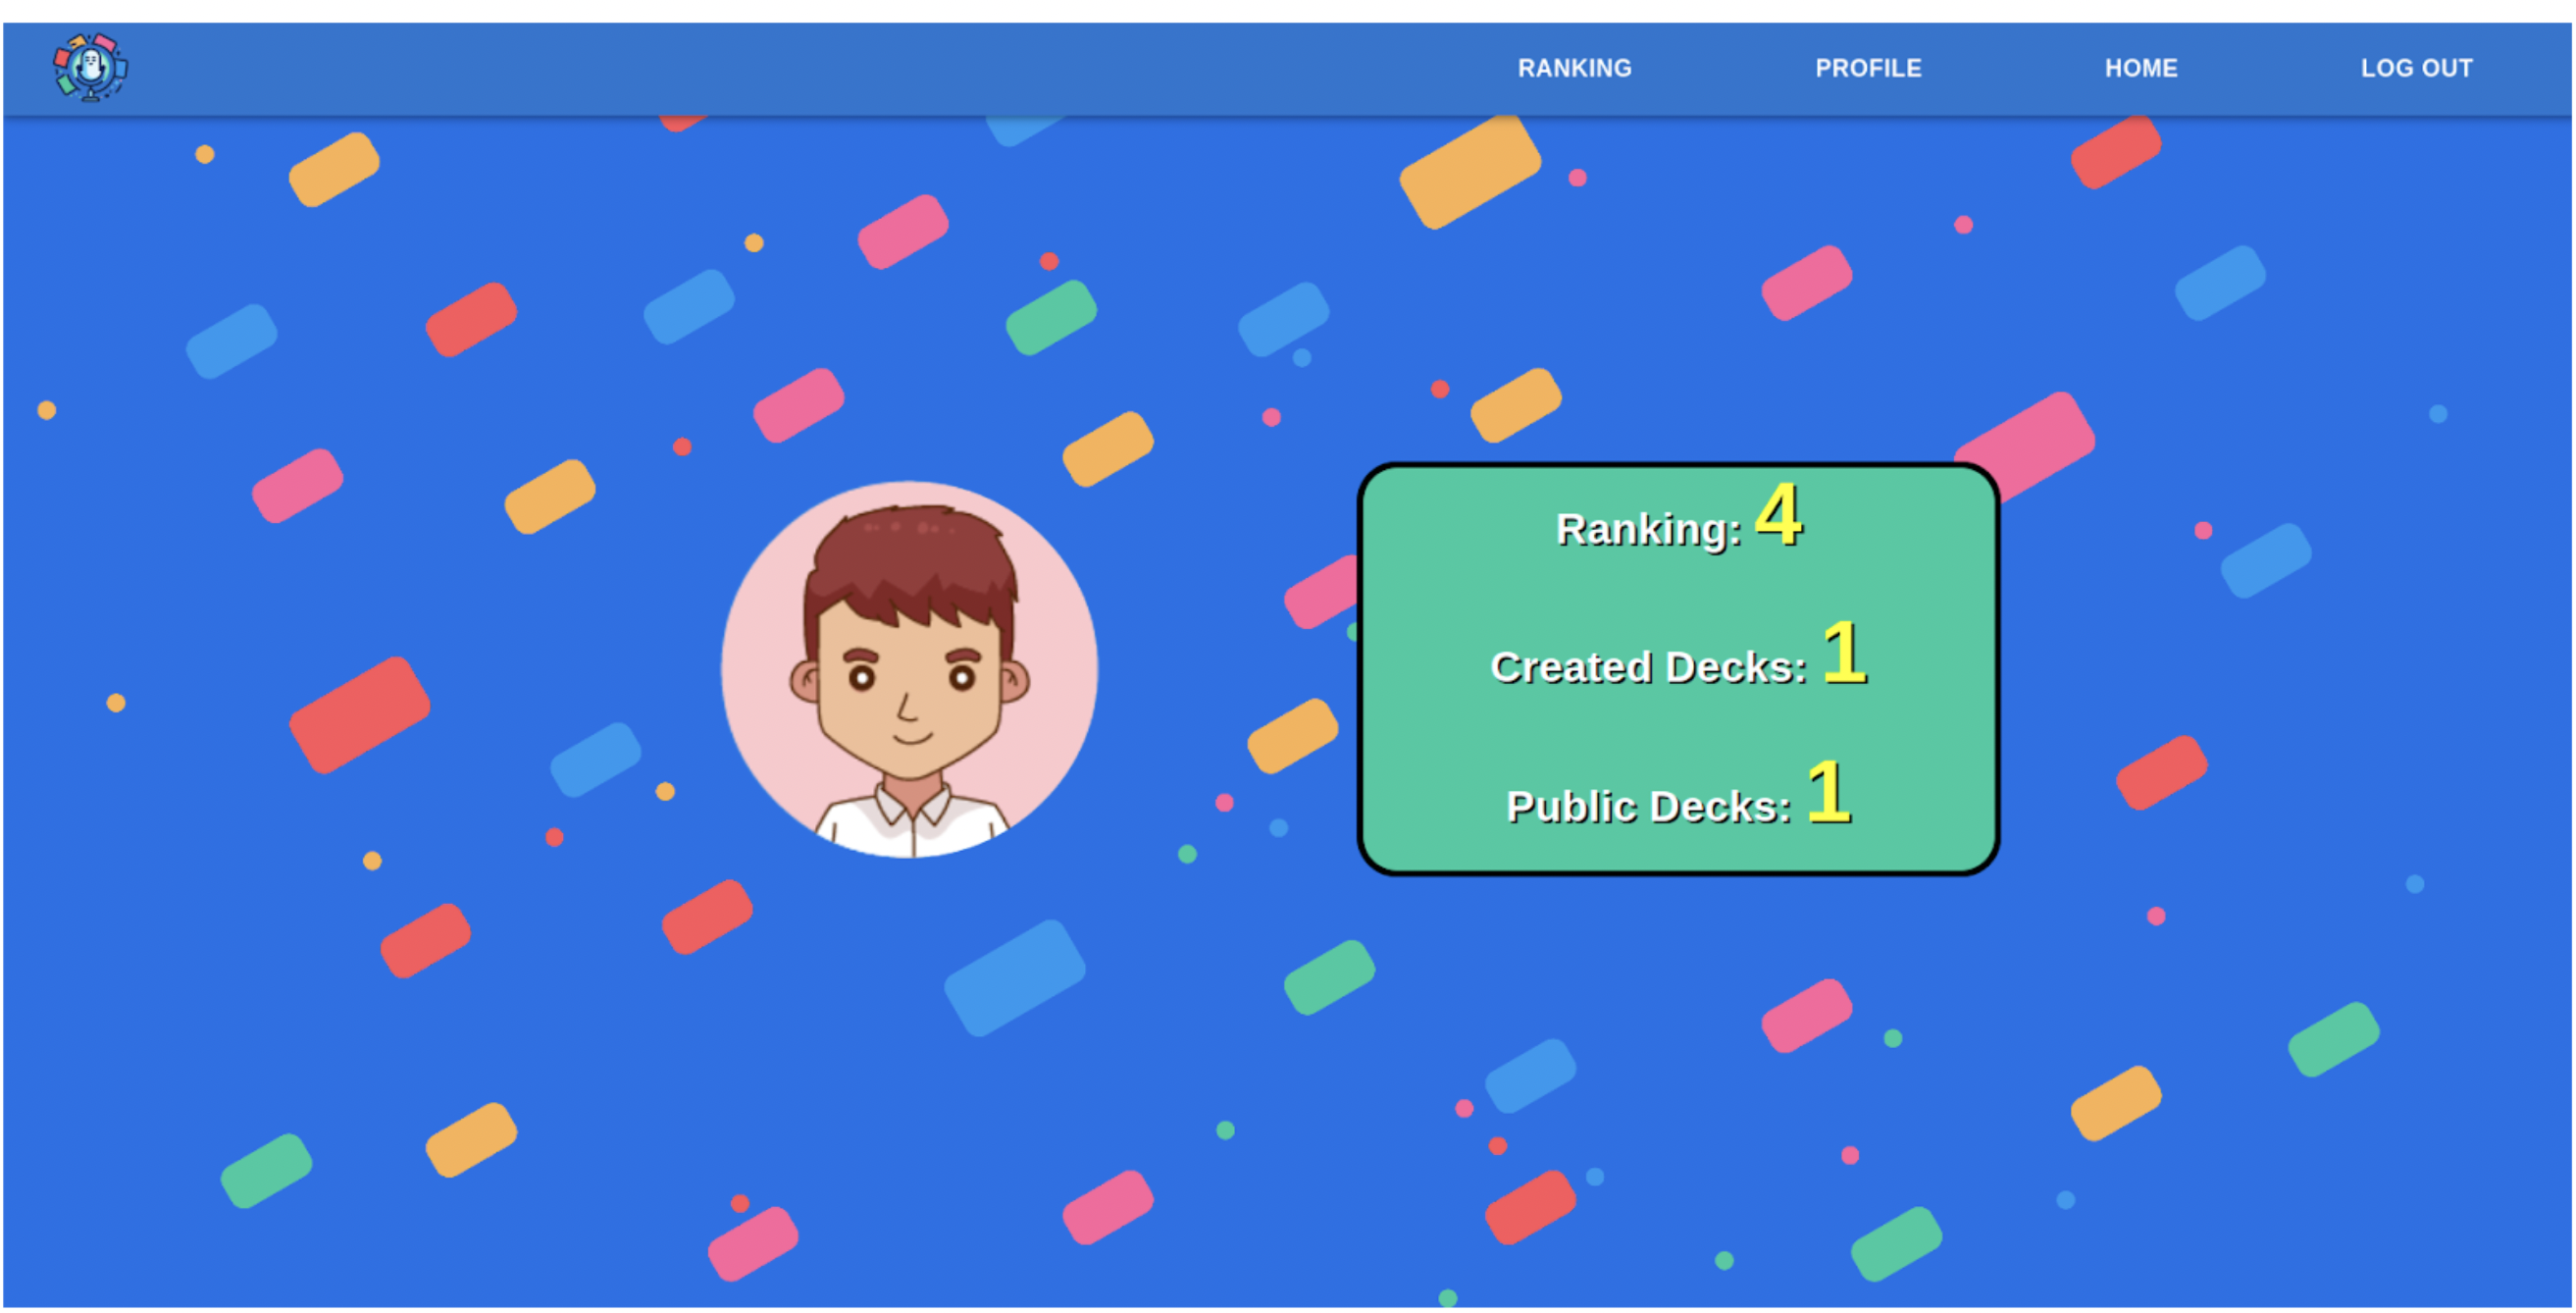
\includegraphics[width=0.9\textwidth]{chapters/chapter_10/images_web/web_stats}
    \caption{Statystyki użytkownika.}
    \label{img:web_stats}
\end{figure}


\subsection{Create deck}
Strona umożliwia tworzenie talii fiszek. Przycisk generate pozwala na wygenerowanie treści fiszki używając chatu gpt. W celu utworzenia talii fiszek użytkownik musi wypełnić nazwę talii, kategorię i mieć przynajmniej jedna wypłenione pole dla fiszki. Przycisk add card dodaje następny formularz do utworzenia fiszki. Użytkownik po wypełnieniu formularza musi kliknąć create deck w celu utworzenia talii.


\begin{figure}[H]
    \centering
    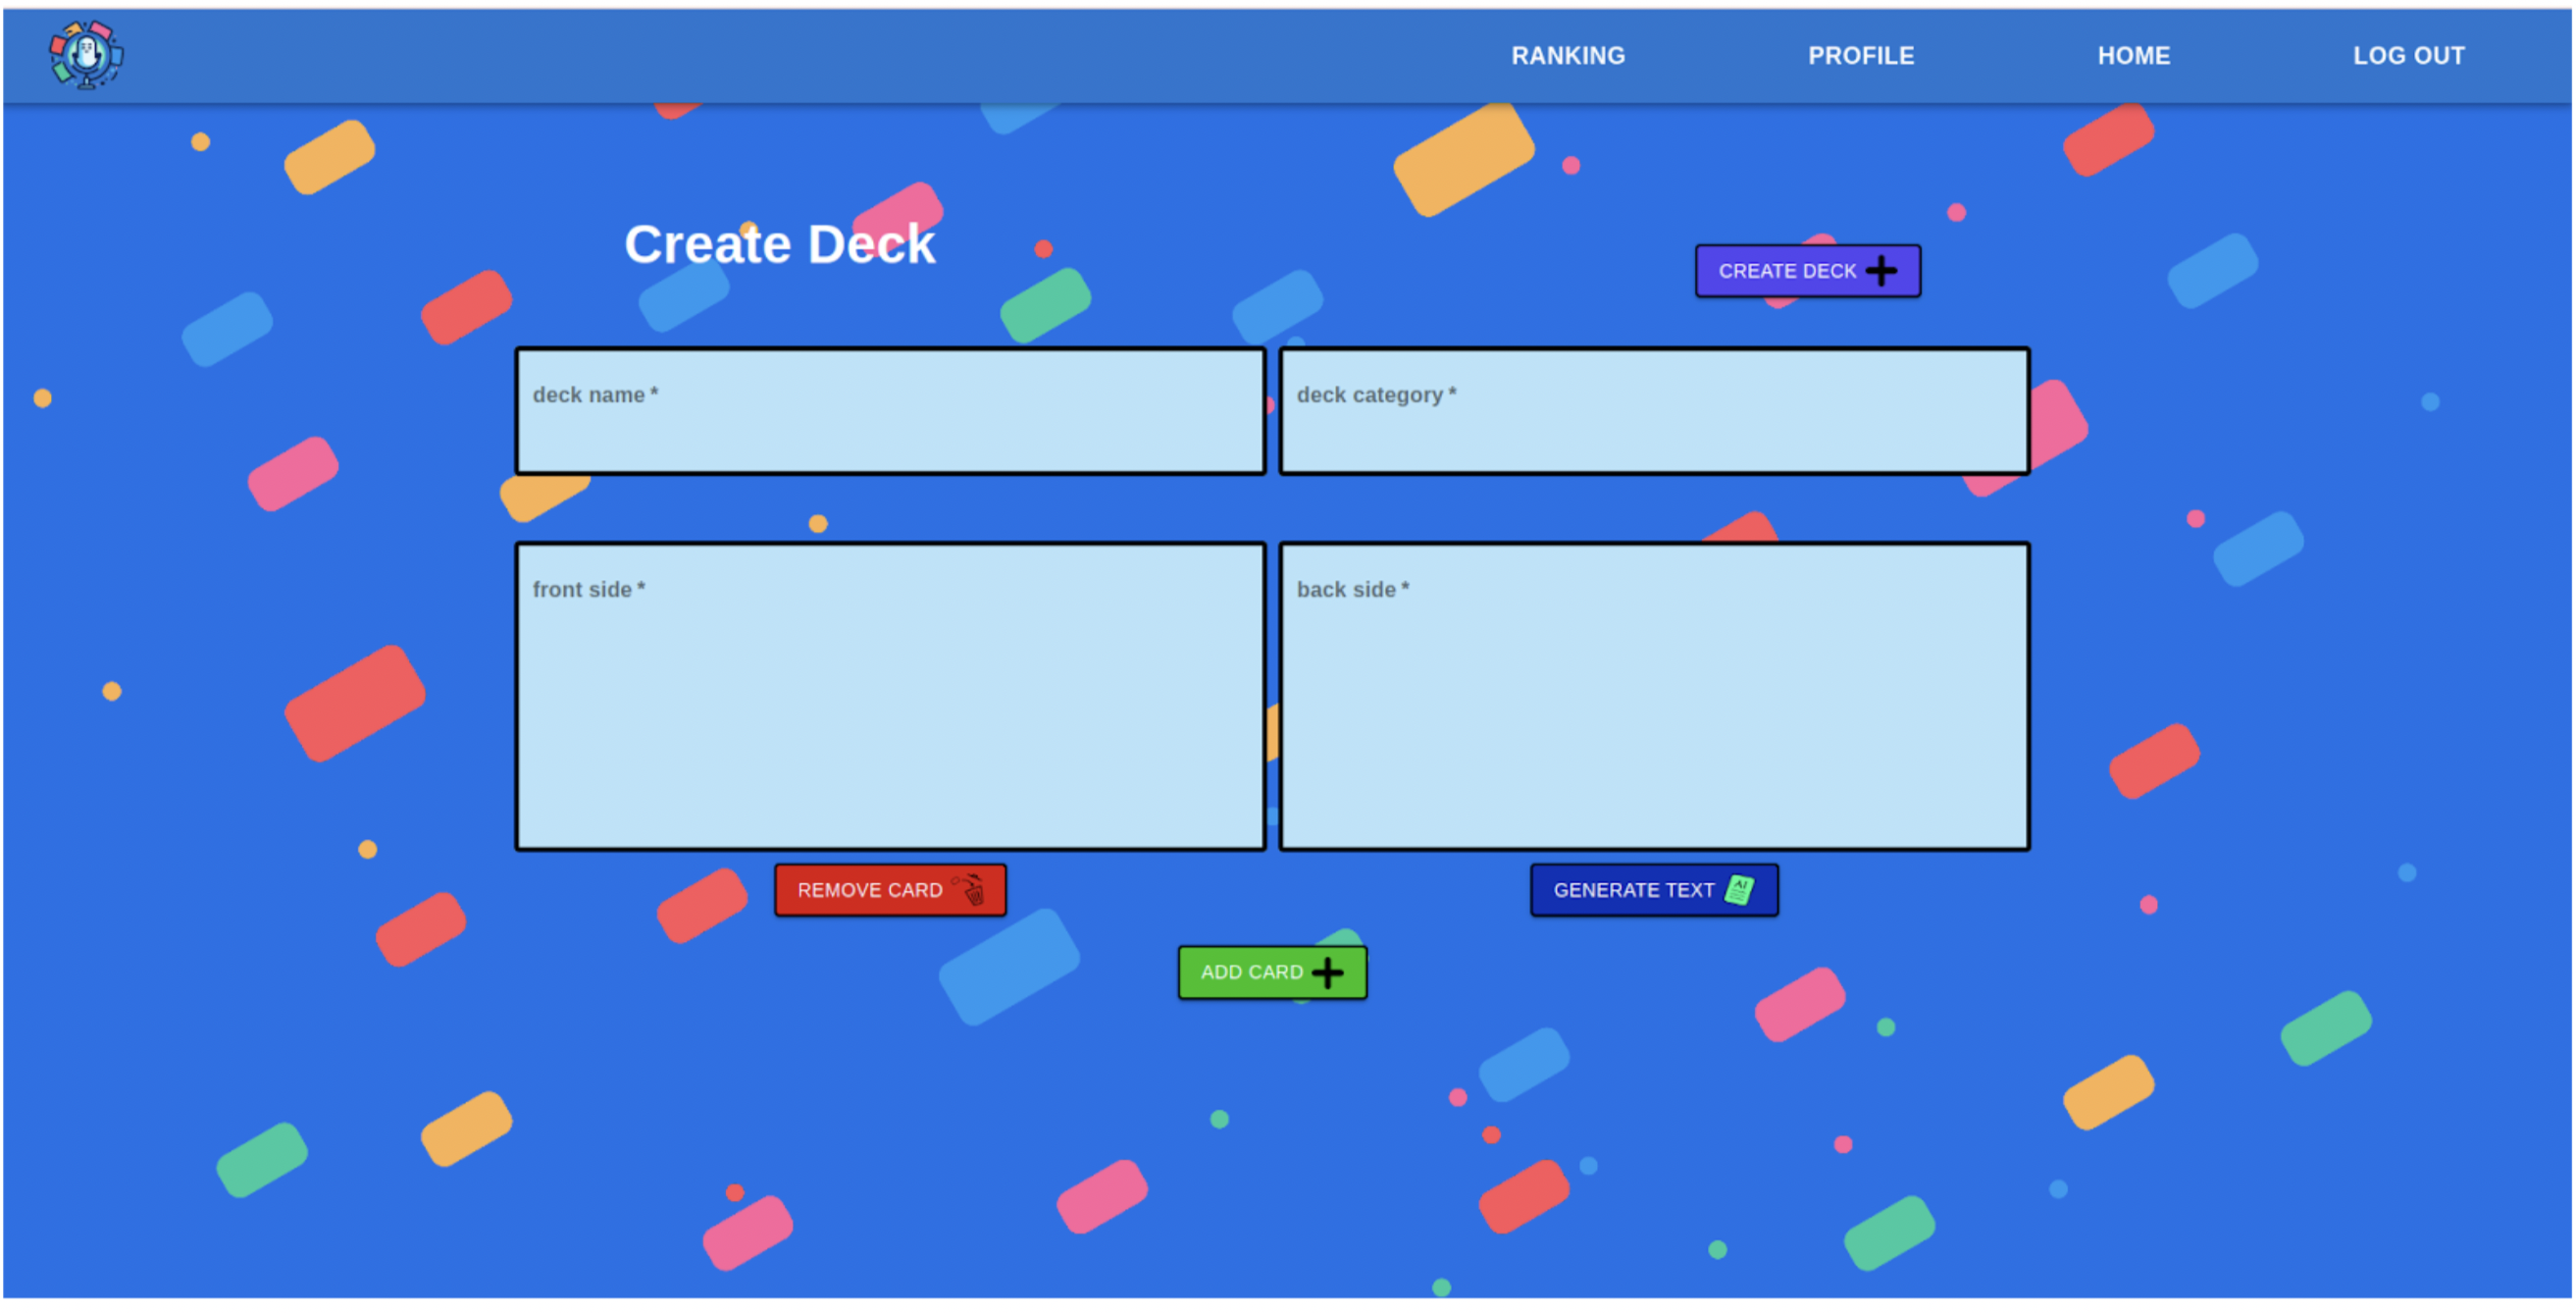
\includegraphics[width=0.9\textwidth]{chapters/chapter_10/images_web/web_create_deck}
    \caption{Widok tworzenia talii.}
    \label{img:web_create_deck}
\end{figure}


Użytkownik może wypełnić przednią stronę fiszki, następnie kliknięcie przycisku generate pozwoli na wygenerowanie przez chat tekstu na podstawie zawartości przedniej strony fiszki. Po wygenerowaniu treść pojawi się w okienku i użytkownik ma możliwość zaakceptowania treści lub jej odrzucenia. W przypadku zaakceptowania tylna strona fiszki zostanie wypełniona wygenerowaną treścią.


\begin{figure}[H]
    \centering
    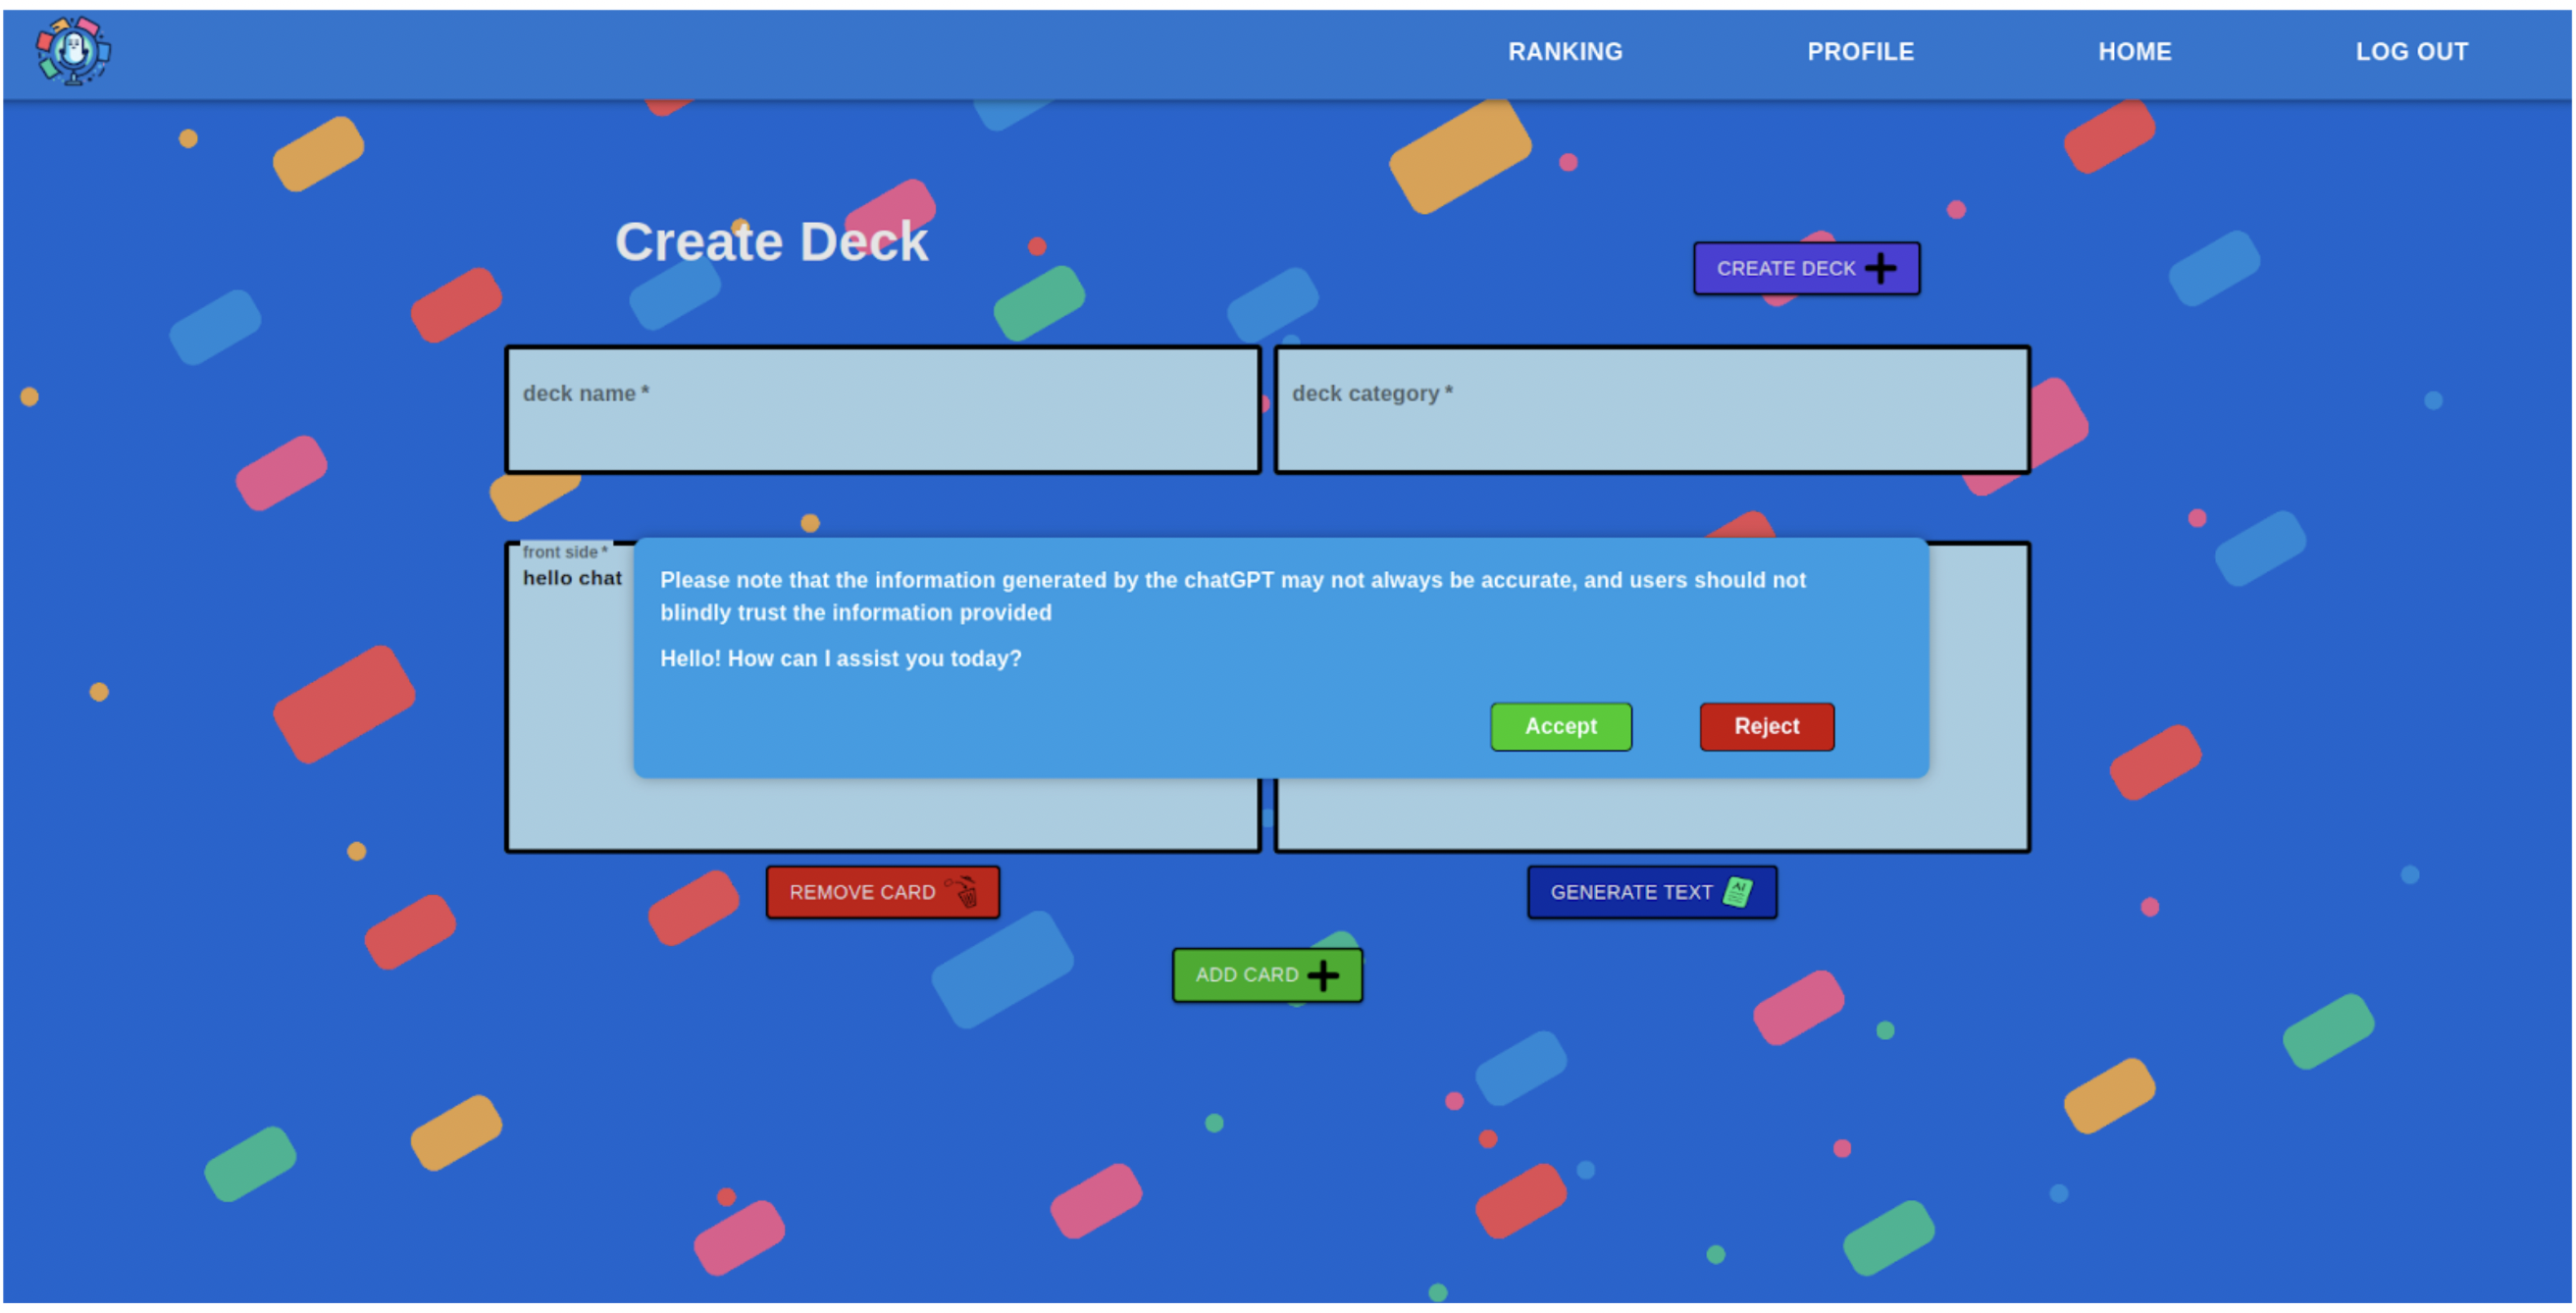
\includegraphics[width=0.9\textwidth]{chapters/chapter_10/images_web/web_chat}
    \caption{Generowanie treści przez ChatGPT.}
    \label{img:web_chat}
\end{figure}


\subsection{My Decks}
W my decks trzymane są wszystkie talie utworzone przez użytkownika. Filter pozwala na filtrowanie decków jednocześnie po kategorii i nazwie talii.


\begin{figure}[H]
    \centering
    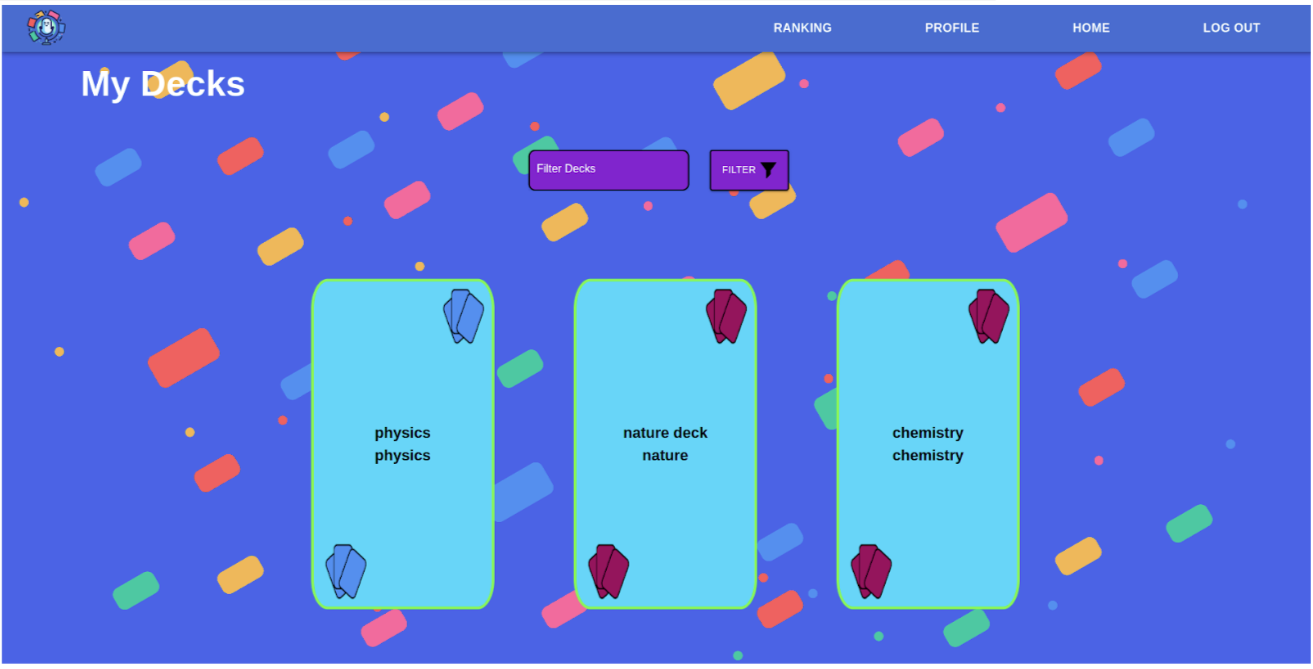
\includegraphics[width=0.9\textwidth]{chapters/chapter_10/images_web/web_my_decks}
    \caption{Widok talii utworzonych przez użytkownika.}
    \label{img:web_my_decks}
\end{figure}


Po otwarciu ukazują się wszystkie fiszki w talii. Użytkownika po kliknięciu learn uruchomien trybu uczenia, który pozwala na podzielenie talii na fiszek na zapamiętane i nie zapamiętane. Memorized to widok w którym widać wszystkie zapamiętane fiszki, a w not memorized znajdują się te nie zapamiętane. W voice control są dostępne wszystkie fiszki do podziału co umożliwia użytkownikowi uruchomienie trybu sterowania na całej dostępnej talii. Opcje oferują użytkownikowi:


\begin{itemize}
    \item udostępnienie talii,
    \item reset talii w celu ustawienia wszystkich fiszek jako niezapamiętane,
    \item usunięcie talii,
    \item dodanie nowej fiszki,
    \item zmianę nazwy lub kategorii talii.
\end{itemize}


\begin{figure}[H]
    \centering
    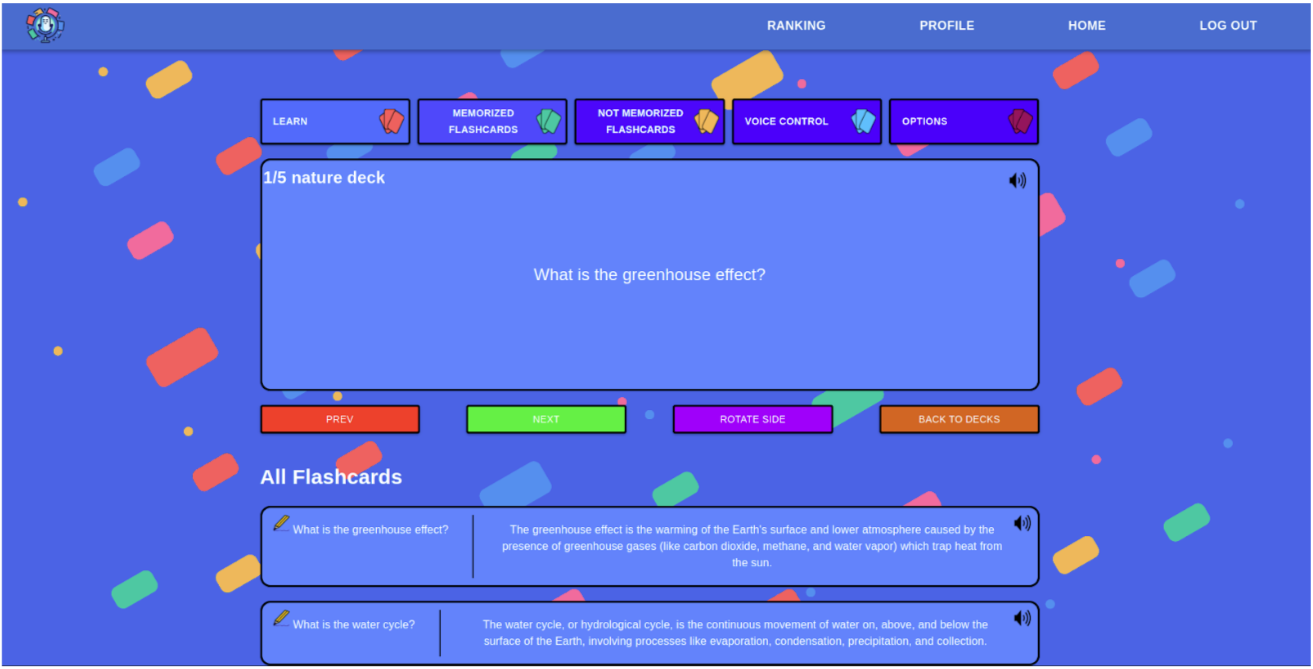
\includegraphics[width=0.9\textwidth]{chapters/chapter_10/images_web/web_deck}
    \caption{Widok talii po jej otworzeniu.}
    \label{img:web_deck}
\end{figure}


\begin{figure}[H]
    \centering
    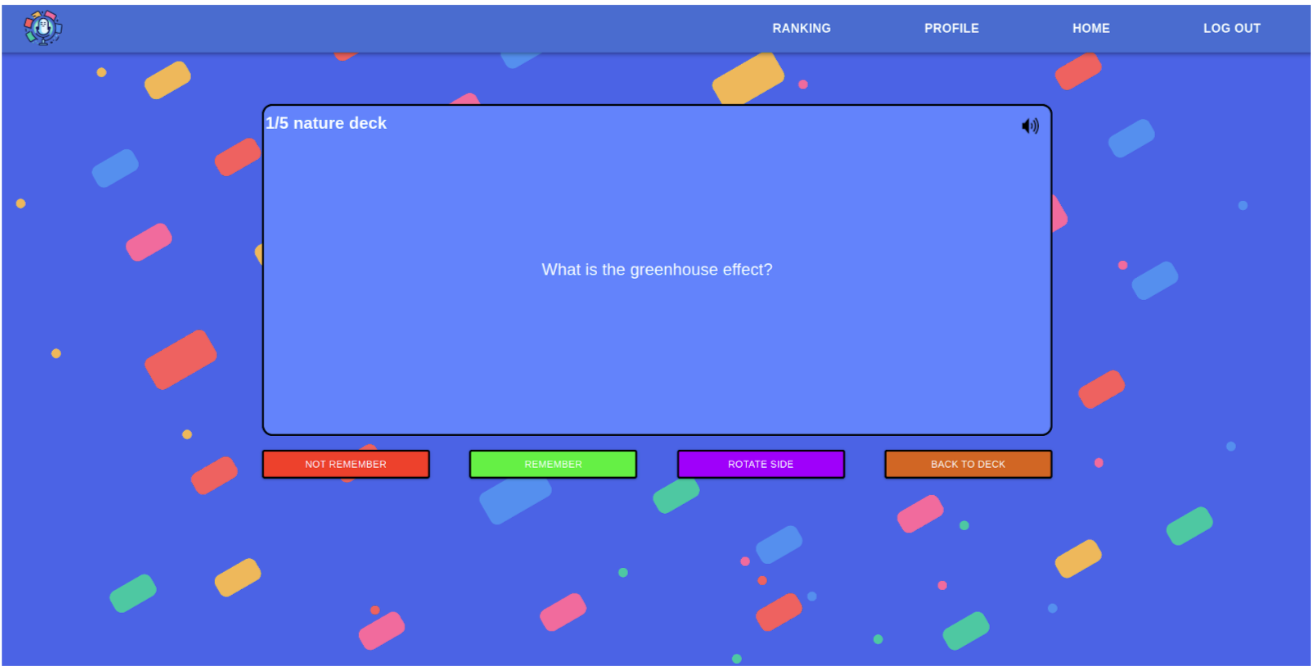
\includegraphics[width=0.9\textwidth]{chapters/chapter_10/images_web/web_learn}
    \caption{Widok podstawowego trybu nauki.}
    \label{img:web_learn}
\end{figure}


\begin{figure}[H]
    \centering
    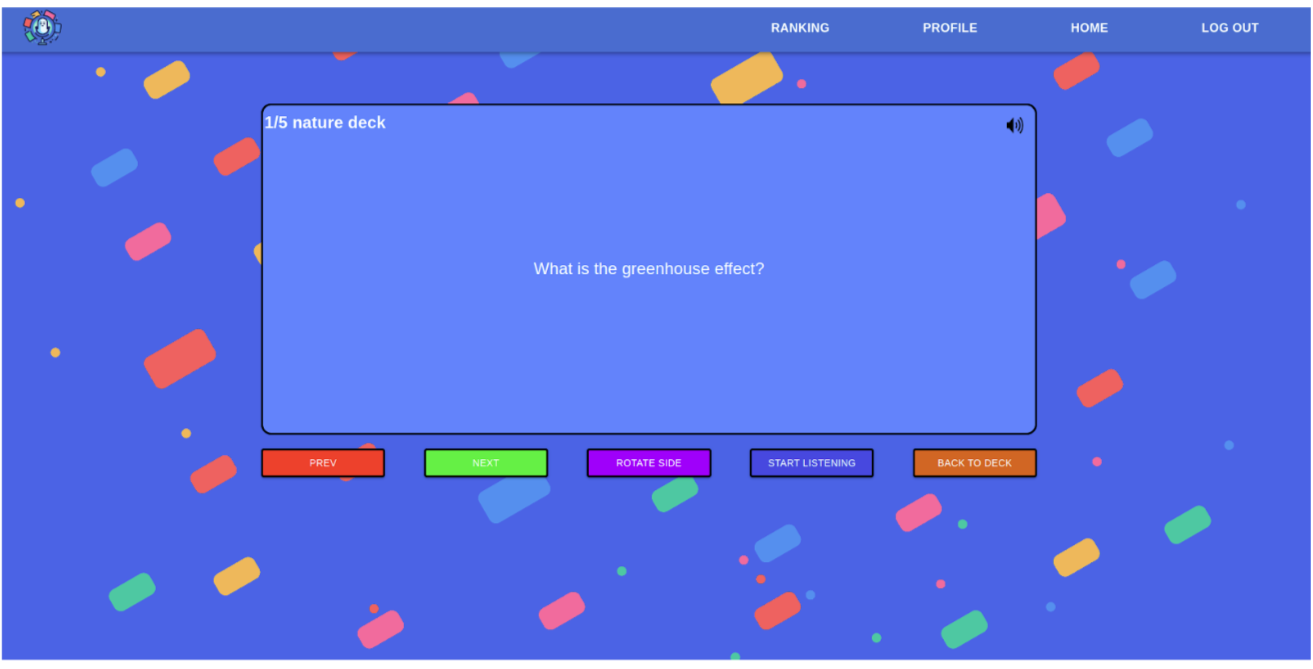
\includegraphics[width=0.9\textwidth]{chapters/chapter_10/images_web/web_voice_1}
    \caption{Widok trybu kontroli głosowej.}
    \label{img:web_voice_1}
\end{figure}


\begin{figure}[H]
    \centering
    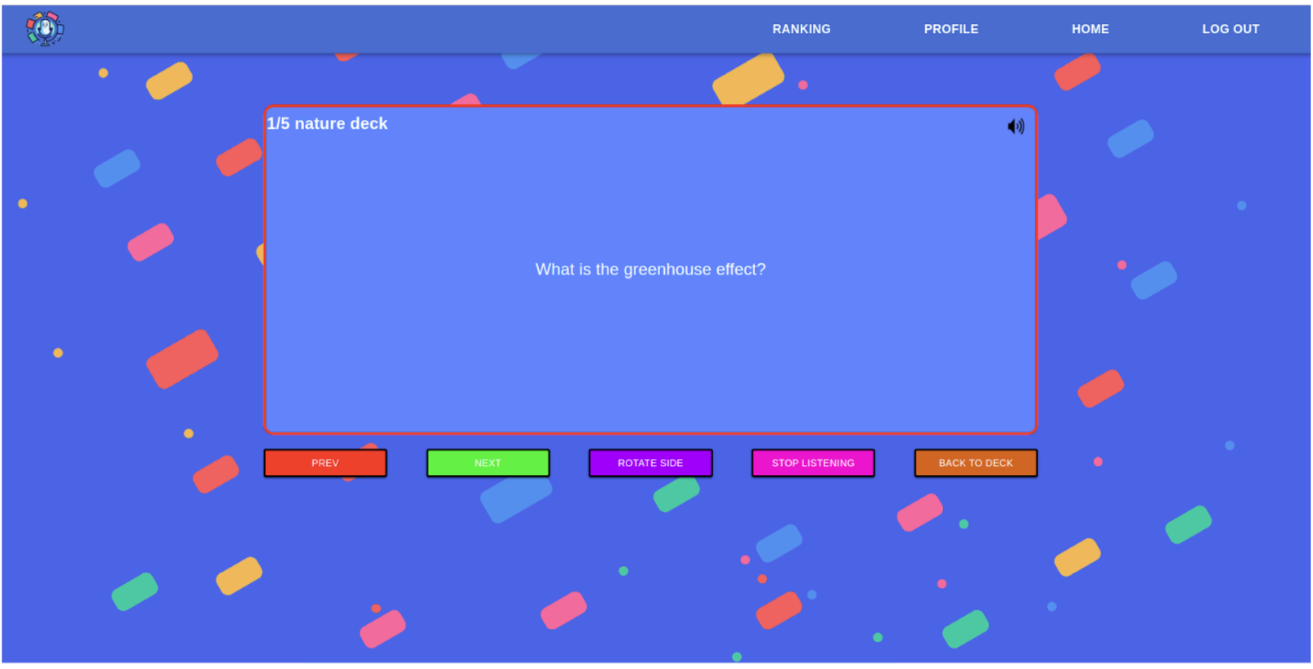
\includegraphics[width=0.9\textwidth]{chapters/chapter_10/images_web/web_voice_2}
    \caption{Widok trybu kontroli głosowej po uruchomieniu.}
    \label{img:web_voice_2}
\end{figure}


\begin{figure}[H]
    \centering
    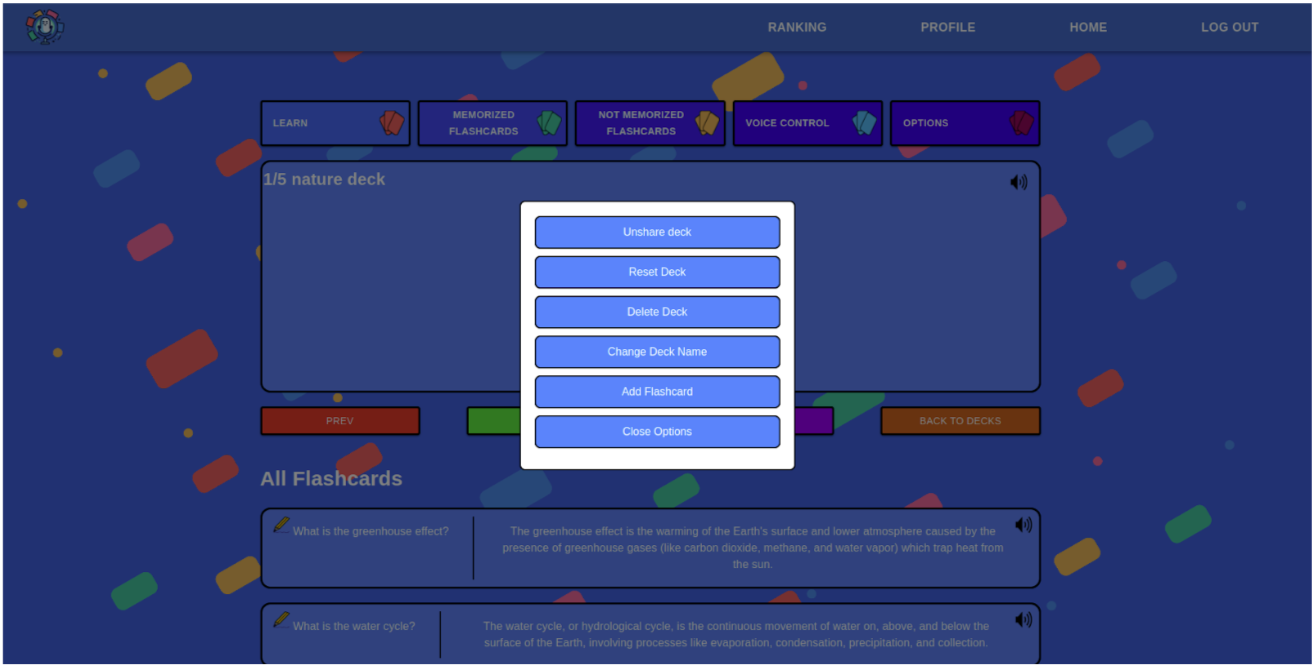
\includegraphics[width=0.9\textwidth]{chapters/chapter_10/images_web/web_settings}
    \caption{Opcje talii.}
    \label{img:web_settings}
\end{figure}


\subsection{Public decks}
Public decks zawiera wszystkie talie, które zostały zaimportowane z rankingu.


\begin{figure}[H]
    \centering
    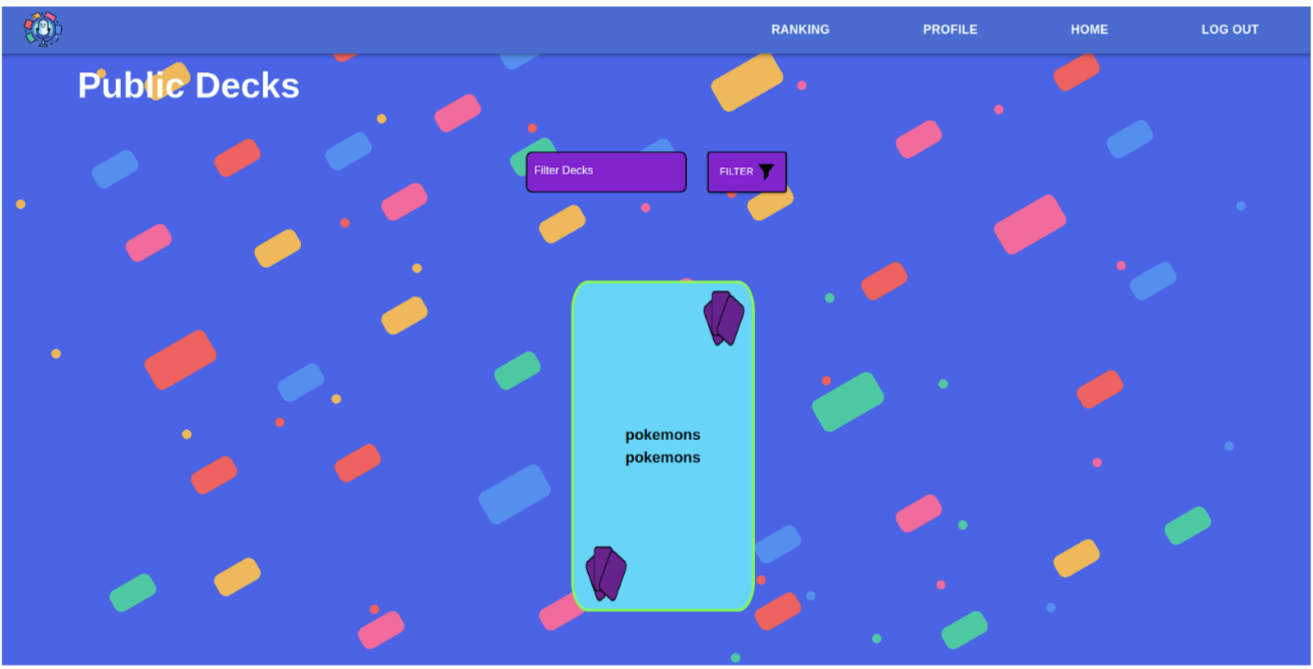
\includegraphics[width=0.9\textwidth]{chapters/chapter_10/images_web/web_public_decks}
    \caption{Widok talii w Public decks.}
    \label{img:web_public_decks}
\end{figure}


\subsection{Ranking użytkowników i talii}
Ranking użytkowników zawiera wszystkie konta, które udostępniły co najmniej jedną talię fiszek. Pozycja w rankingu jest zależna od sumy pobrań wszystkich talii udostępnionych przez użytkownika.


\begin{figure}[H]
    \centering
    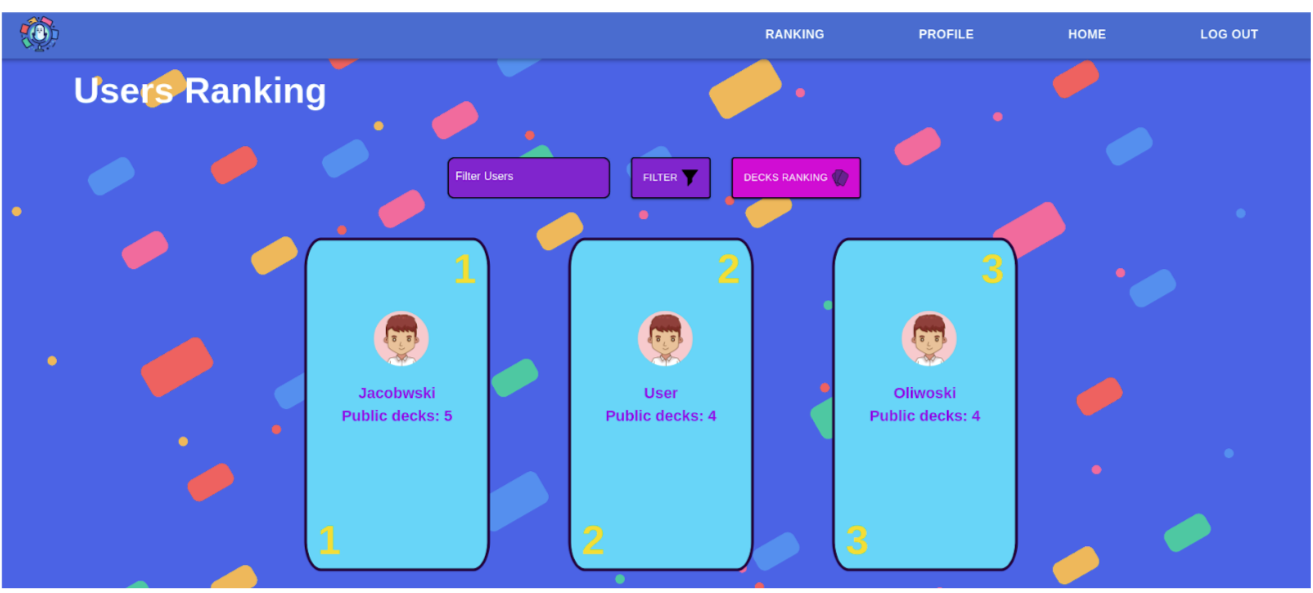
\includegraphics[width=0.9\textwidth]{chapters/chapter_10/images_web/web_user_ranking}
    \caption{Ranking użytkowników.}
    \label{img:web_user_ranking}
\end{figure}


\begin{figure}[H]
    \centering
    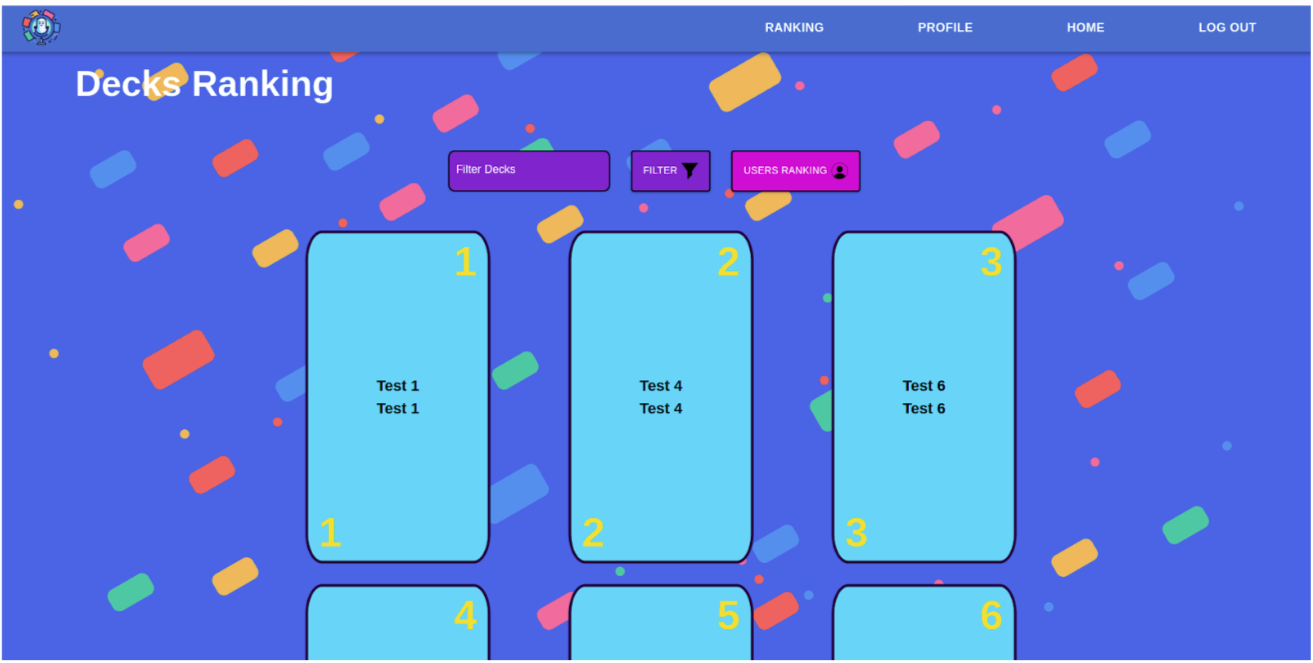
\includegraphics[width=0.9\textwidth]{chapters/chapter_10/images_web/web_decks_ranking}
    \caption{Ranking publicznych talii.}
    \label{img:web_decks_ranking}
\end{figure}


Użytkownik po otwarciu konkretnej talii ma możliwość obejrzenia jej zawartości. Jeżeli talia spodoba się użytkownikowi ma ona możliwość zaimportowania jej i w ten sposób talia zostanie dodana do public decks. Można także zgłosić talię w przypadku gdy zawiera ona wulgaryzmy lub inne nieprzyzwoite wyrażenia. Po zgłoszeniu talii moderator widzi taką talię w zgłoszeniach.


\begin{figure}[H]
    \centering
    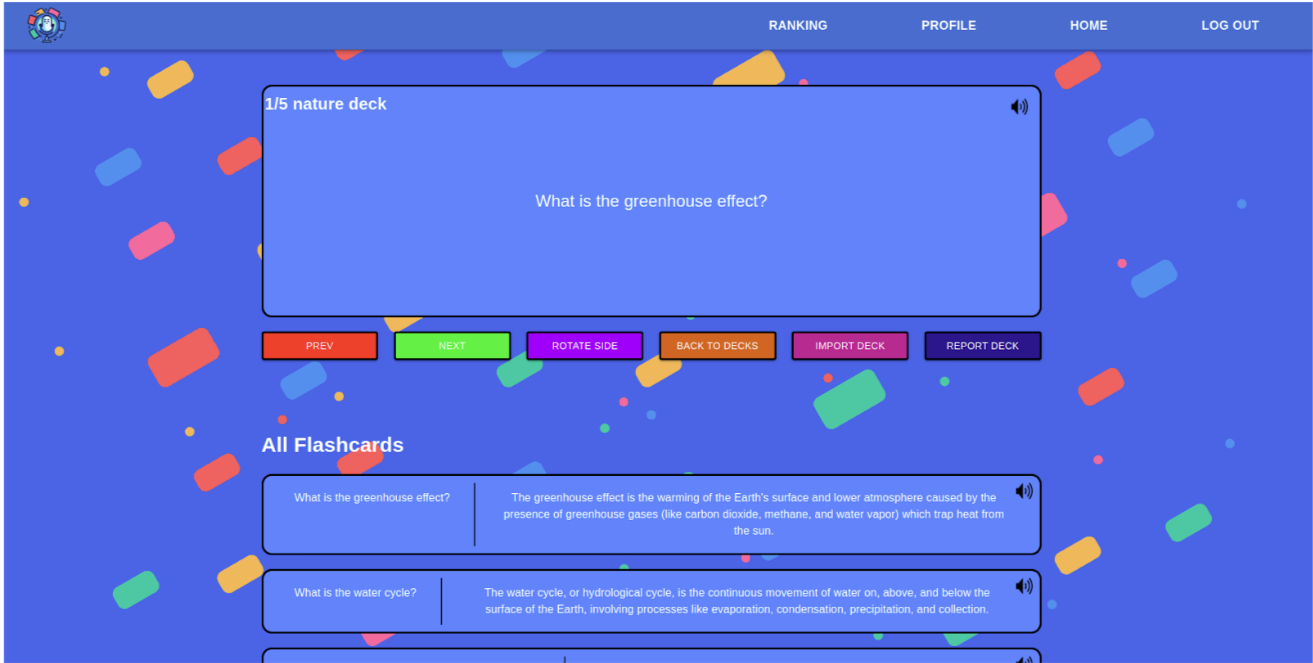
\includegraphics[width=0.9\textwidth]{chapters/chapter_10/images_web/web_public_deck}
    \caption{Widok talii wybranej z rankingu.}
    \label{img:web_public_deck}
\end{figure}

\subsection{Panel moderatora}
Panel moderatora pozwala na usuwanie użytkowników, usuwanie talii lub edycję fiszek lub ich usunięcie. Do panelu moderatora mogą przejść tylko osoby z kontem moderatora, użytkownikom z takim kontem w profilu pojawia się dodatkowy przycisk przekierowujący do panelu moderatora.


\begin{figure}[H]
    \centering
    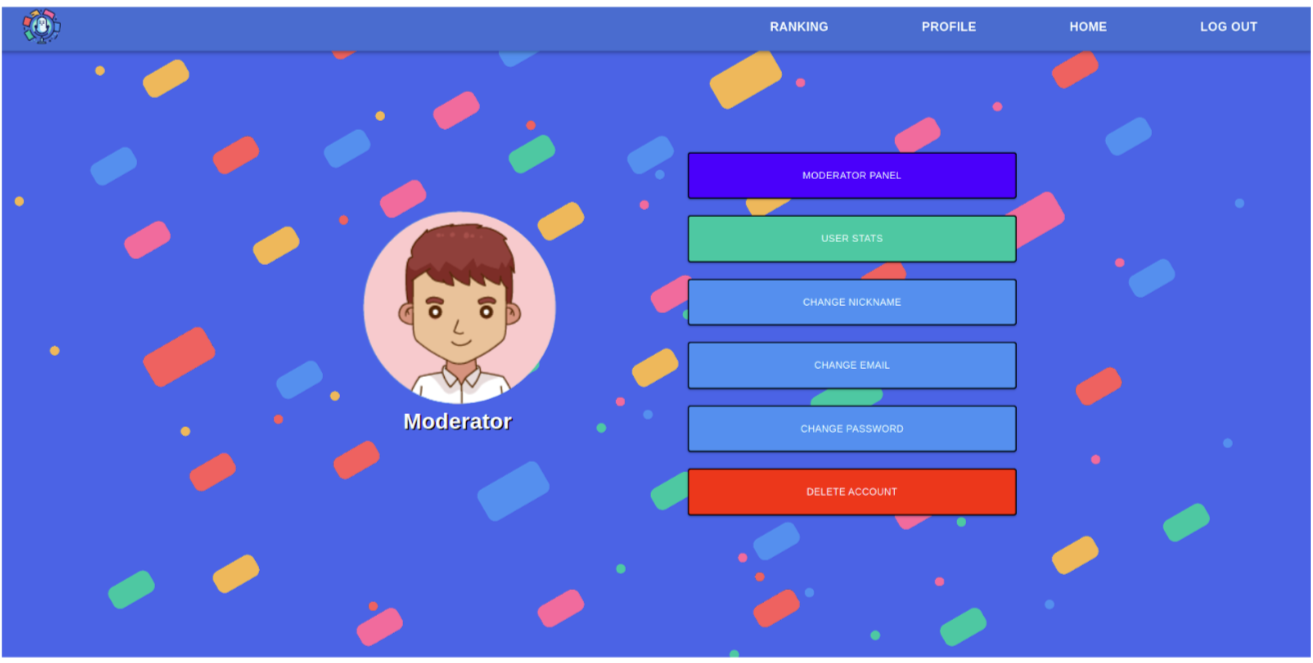
\includegraphics[width=0.9\textwidth]{chapters/chapter_10/images_web/web_moderator_profile}
    \caption{Profil użytkownika konta moderatora.}
    \label{img:web_moderator_profile}
\end{figure}


\begin{figure}[H]
    \centering
    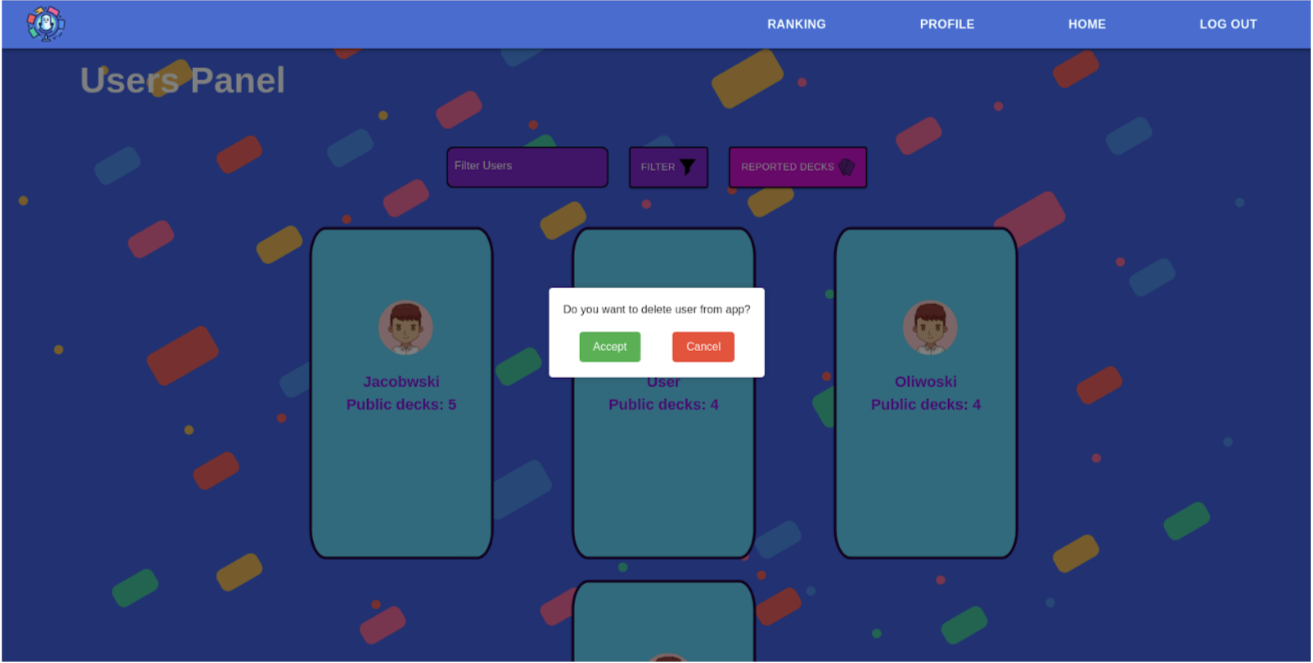
\includegraphics[width=0.9\textwidth]{chapters/chapter_10/images_web/web_moderator_delete_user}
    \caption{Usunięcie użytkownika przez moderatora.}
    \label{img:web_moderator_delete_user}
\end{figure}


\begin{figure}[H]
    \centering
    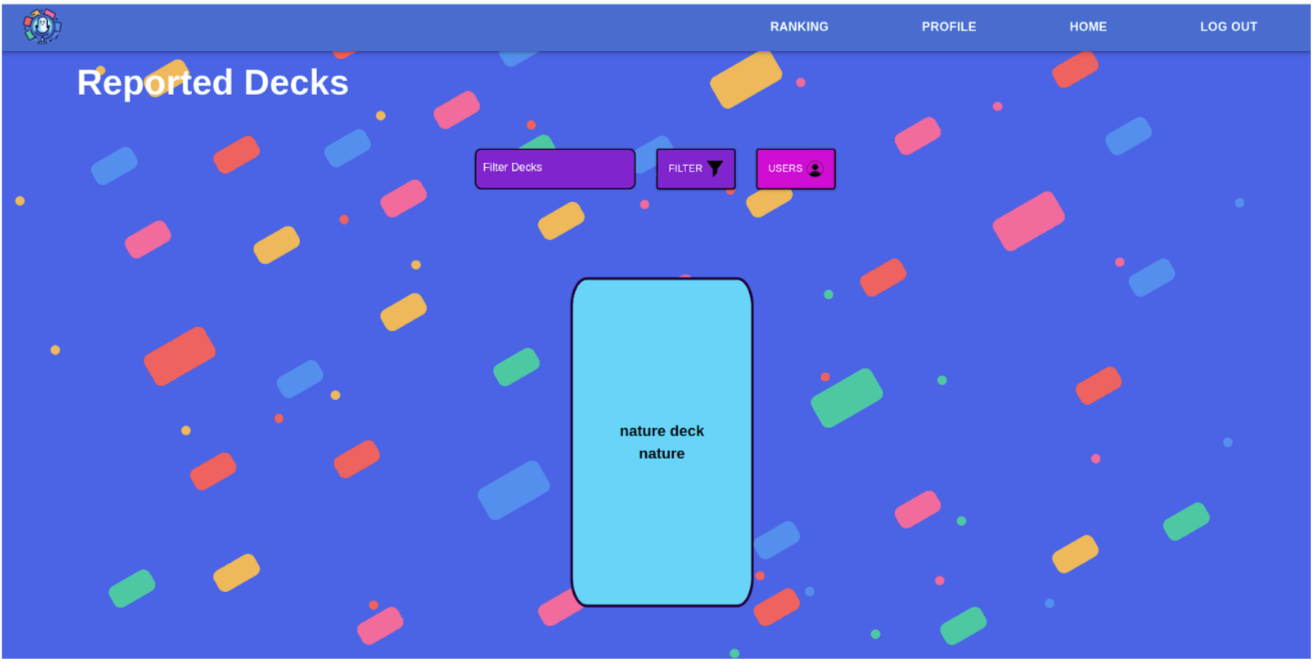
\includegraphics[width=0.9\textwidth]{chapters/chapter_10/images_web/web_reported_decks}
    \caption{Widok zgłoszonych talii.}
    \label{img:web_reported_decks}
\end{figure}


Moderator po otwarciu talii może ją przejrzeć w celu sprawdzenia czy report talii był uzasadniony w przypadku gdy report talii był nie potrzebny może usunąć ją z listy zgłoszeń. Jeżeli zgłoszenie było prawidłowe może usunąć talię z aplikacji.


\begin{figure}[H]
    \centering
    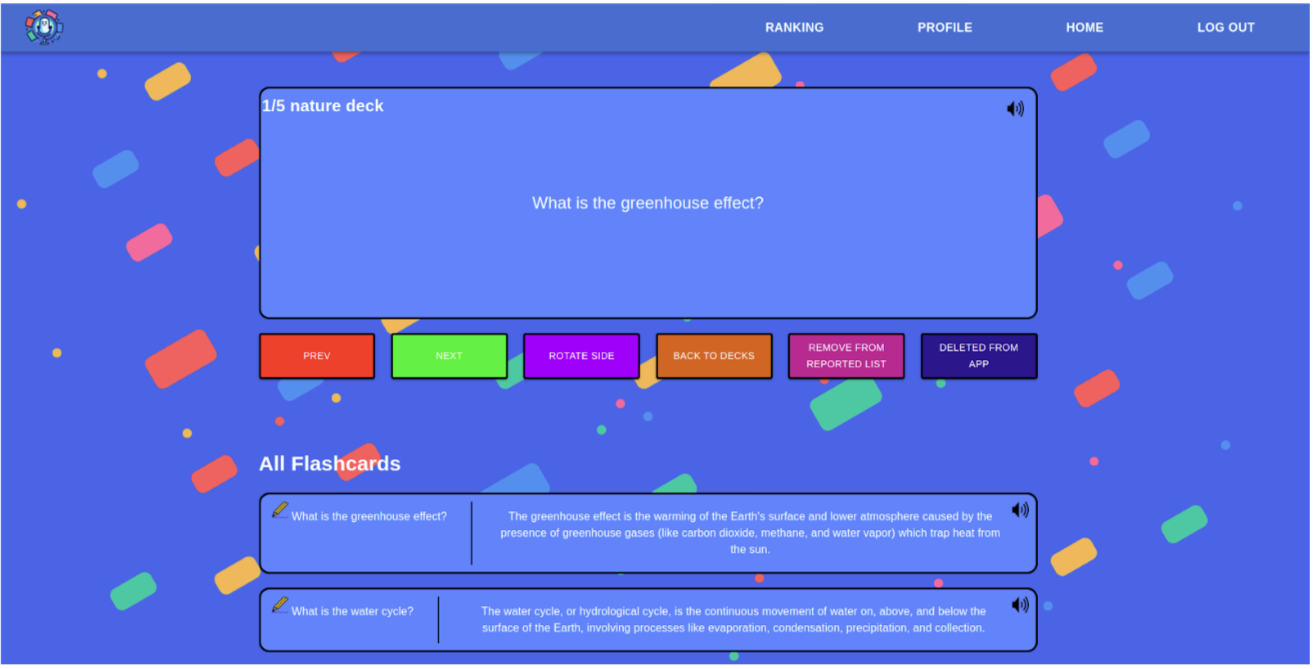
\includegraphics[width=0.9\textwidth]{chapters/chapter_10/images_web/web_reported_deck_2}
    \caption{Widok zgłoszonej talii.}
    \label{img:web_reported_deck_2}
\end{figure}